\documentclass[10pt,a4paper,twocolumn]{article}

\usepackage{amsmath,amssymb}
\usepackage{graphicx}
\usepackage{booktabs}
\usepackage{array}
\usepackage{multirow}
\usepackage[colorlinks=true,linkcolor=blue,citecolor=blue,urlcolor=blue]{hyperref}
\usepackage{caption}
\usepackage{subcaption}
\usepackage{natbib}
\usepackage[top=0.73in,bottom=0.73in,left=0.58in,right=0.58in,columnsep=0.20in]{geometry}
\usepackage{microtype}
\usepackage{placeins}
\usepackage{titlesec}
\usepackage{setspace}

% Section / subsection heading spacing
\titlespacing*{\section}{0pt}{8pt plus 2pt minus 1pt}{4pt plus 1pt}
\titlespacing*{\subsection}{0pt}{6pt plus 2pt minus 1pt}{3pt plus 1pt}
\titlespacing*{\subsubsection}{0pt}{4pt}{2pt}

% Float and caption spacing
\setlength{\textfloatsep}{5pt plus 1pt minus 1pt}
\setlength{\floatsep}{4pt plus 1pt minus 1pt}
\setlength{\intextsep}{4pt plus 1pt minus 1pt}
\setlength{\abovecaptionskip}{2pt}
\setlength{\belowcaptionskip}{1pt}

% Equation display spacing
\setlength{\abovedisplayskip}{5pt plus 2pt minus 2pt}
\setlength{\belowdisplayskip}{5pt plus 2pt minus 2pt}
\setlength{\abovedisplayshortskip}{3pt plus 1pt}
\setlength{\belowdisplayshortskip}{3pt plus 1pt}

% Caption font size
\captionsetup{font=footnotesize,labelfont=bf}

% Bibliography entry spacing
\setlength{\bibsep}{2pt}

\title{\textbf{Beyond Binary: Four-Class Risk Stratification from\\
Gastrointestinal Endoscopy Using Asymmetric-Cost\\
Lightweight CNN--Transformer Learning\\
and Demographic Equity Analysis}}

\author{%
  Azizur Rahman$^{1}$ \and
  Nakib Uddin Ahmed$^{2}$ \and
  Mehjabin Ferdous$^{3}$ \and
  Kadirur Rahman Chowdhury$^{4}$
}

\newcommand{\authoraffils}{%
  \small
  $^{1}$Department of CAPS (Computer Technology),
  Indiana Wesleyan University, Marion, IN 46953, USA.
  \texttt{azizurusa22@gmail.com}\\[2pt]
  $^{2}$Department of Computer Science and Engineering,
  Metropolitan University, Bateshwar, Sylhet, Bangladesh.
  \texttt{nakibuddin33@gmail.com}\\[2pt]
  $^{3}$Masters in Public Health (MPH),
  St.\ Francis College, 179 Livingstone St, Brooklyn, NY 11201, USA.
  \texttt{mehjabinferdousmu@gmail.com}\\[2pt]
  $^{4}$Birmingham City Business School, Faculty of Business, Law and Social Sciences,
  Birmingham City University, Birmingham B4 7BD, United Kingdom.
  \texttt{kadirurrahmanchowdhury@gmail.com}
}

\date{}

\begin{document}

\twocolumn[{%
\maketitle
\begin{@twocolumnfalse}
\noindent\authoraffils
\vspace{3pt}
\begin{abstract}
Gastrointestinal (GI) cancers account for over 3.5 million deaths annually,
yet existing AI-assisted endoscopy systems reduce the clinical decision to a
binary lesion-present/absent output that is misaligned with actionable
clinical practice guidelines and provides no guidance on intervention urgency.
We present the first lightweight CNN--Transformer benchmark for four-class GI
lesion \emph{risk stratification} aligned with American College of
Gastroenterology (ACG) and European Society of Gastrointestinal Endoscopy
(ESGE) guidelines. We map 23 HyperKvasir finding classes to four clinically
actionable risk tiers---Normal (routine surveillance), Inflammatory (medical
management), Pre-malignant (biopsy required), and High-Risk (immediate
intervention)---and train three lightweight architectures (DenseNet-121,
EfficientNet-B0, DeiT-Tiny; all $<$8\,M parameters) under a novel
\textbf{Asymmetric Endoscopy Loss (AEL)} that assigns a 5$\times$
misclassification penalty to High-Risk lesions, reflecting the clinical
reality that missed High-Risk lesions reduce five-year survival from 90\% to
under 20\%. Contrast-Limited Adaptive Histogram Equalisation (CLAHE)
preprocessing enhances mucosal contrast prior to augmentation. Cross-dataset
generalisation is validated zero-shot on the independent Kvasir-v2 cohort.
GradCAM heatmaps localise clinically relevant mucosal features per risk tier,
Monte Carlo Dropout uncertainty quantification flags borderline cases for
mandatory endoscopist review, and we introduce a Cross-Demographic
Consistency of Tier-level Equity Index (CD-CTEI) as a methodological
framework for auditing prediction fairness across demographic subgroups,
demonstrated here on synthetic proxy subgroups in the absence of annotated
patient demographics. The best model (EfficientNet-B0) reaches macro
F1\,$=$\,0.83 on HyperKvasir and 0.76 zero-shot on Kvasir-v2, with 43.9\,\%
workload reduction and zero missed High-Risk cases across all architectures.
\end{abstract}

\noindent\textbf{Keywords:}
Gastrointestinal endoscopy;
Risk stratification;
Asymmetric loss function;
Lightweight neural networks;
Vision Transformer;
DenseNet;
EfficientNet;
GradCAM;
Monte Carlo Dropout;
Clinical equity;
HyperKvasir
\end{@twocolumnfalse}
}]

%% ============================================================================
\section{Introduction}
\label{sec:intro}
%% ============================================================================

Gastrointestinal cancers---encompassing colorectal, gastric, and oesophageal
malignancies---collectively account for more than 3.5 million deaths annually
and represent the second leading cause of cancer mortality
worldwide~\citep{Sung2021}. Early-stage lesions are missed in up to 26\,\% of
endoscopic procedures due to subtle mucosal changes, inter-endoscopist
variability, and endoscopist fatigue during high-volume screening
sessions~\citep{Kaminski2017}. Computer-aided detection (CAD) systems have
demonstrated statistically significant improvements in polyp detection in
randomised controlled trials~\citep{Wang2019}, leading to regulatory approval
of the first AI endoscopy devices. However, the clinical utility of deployed
CAD systems remains constrained by a fundamental design mismatch: virtually
all systems reduce the endoscopic decision to a binary lesion-present or
lesion-absent output~\citep{Pogorelov2017}.

This binary framing does not correspond to any published clinical practice
guideline. Both the ACG and the ESGE classify GI findings into tiered risk
categories that map to distinct clinical actions: routine surveillance
intervals for normal mucosa, medical management for inflammatory lesions,
mandatory biopsy and intensified surveillance for pre-malignant findings, and
immediate endoscopic resection or oncology referral for high-risk
lesions~\citep{Shaukat2021,Ferlitsch2017}. A binary AI output cannot guide
these decisions, reducing the technology to a simple alert with no actionable
resolution. Binary systems also apply identical classification costs
to all errors, ignoring the critical asymmetry in clinical consequences: a
missed High-Risk lesion may progress to invasive cancer within months, while
over-triaging a Normal finding results only in an unnecessary repeat
procedure~\citep{Rawla2019}.

Prior deep learning work on GI endoscopy has focused predominantly on polyp
detection~\citep{Tajbakhsh2016} and binary lesion
classification~\citep{Pogorelov2017}. Multi-class staging has been explored
in isolated contexts, such as Barrett's oesophagus severity
grading~\citep{Ebigbo2019}, but no prior work has framed the problem as a
unified four-class risk stratification aligned with ACG/ESGE guidelines
across the entire GI tract. Compact Vision Transformers, specifically
DeiT-Tiny~\citep{Touvron2021} with 5.9\,M parameters, enable global mucosal
context modelling through patch token self-attention without the 86\,M$+$
parameter cost of full ViT~\citep{Dosovitskiy2021}, making them deployable on
clinical-grade hardware. On the loss side, Focal Loss~\citep{Lin2017}
addresses class imbalance by down-weighting easy examples but does not encode
inter-class \emph{risk} asymmetry---the clinically critical distinction
between missing a Normal finding and missing a High-Risk lesion.

We reframe the problem as \emph{four-class risk stratification} aligned
with published ACG/ESGE intervention thresholds rather than binary
lesion presence. The core technical contribution is the
\textbf{Asymmetric Endoscopy Loss (AEL)}, a weighted cross-entropy
formulation that assigns a 5$\times$ penalty to High-Risk
misclassification, encoding the survival cost asymmetry directly into
the training objective. We benchmark three lightweight architectures
($<$8\,M parameters each: DenseNet-121, EfficientNet-B0, DeiT-Tiny)
under identical conditions, evaluate zero-shot generalisation on the
independent Kvasir-v2 cohort, and pair predictions with Monte Carlo
Dropout uncertainty quantification to construct a referral protocol
that structurally guarantees zero missed High-Risk lesions. GradCAM
saliency maps provide per-class explainability for clinical audit, an
ablation isolates the contribution of AEL against cross-entropy and
Focal Loss, and we propose a Cross-Demographic Consistency of Tier-level
Equity Index (CD-CTEI) as a reusable framework for quantifying prediction
fairness across demographic subgroups once annotated patient demographics
become available. To our knowledge, this is the first work to frame GI
endoscopy AI as guideline-aligned four-class risk stratification rather than
binary lesion detection, evaluated under a uniform sub-8\,M parameter budget
across both convolutional and transformer architectures. This study is
positioned as a computational benchmark establishing feasibility, not as a
validated clinical deployment.

%% ============================================================================
\section{Methods}
\label{sec:methods}
%% ============================================================================

\subsection{Datasets}
\label{sec:datasets}

We used HyperKvasir~\citep{Borgli2020} as the primary training and evaluation
dataset. HyperKvasir is the largest publicly available annotated GI endoscopy
dataset, comprising 110,079 images from both upper and lower GI tract
examinations collected at Baerum Hospital, Norway. The labelled image subset
contains 10,662 images across 23 finding classes, organised in a nested
directory structure by GI tract region, anatomical category, and finding
class. Each class folder contains JPEG images of variable resolution,
standardised to $224\times224$ pixels prior to training.

For external validation, we used Kvasir-v2~\citep{Pogorelov2017b}, an
independent dataset of 8,000 images across 8 GI finding classes collected
from a different patient population and imaging equipment. Kvasir-v2 was used
exclusively for zero-shot evaluation---no Kvasir-v2 images were used during
training or hyperparameter selection. This design tests the ability of models
trained on HyperKvasir to generalise to a clinically and technically distinct
cohort.

The full dataset was split at the image level with stratified sampling into
training (70\%), validation (15\%), and test (15\%) sets, with reproducibility
ensured by a fixed random seed (SEED\,$=$\,42). The training set was further
balanced using \texttt{WeightedRandomSampler} with weights inversely
proportional to class frequencies, ensuring equal expected class
representation per batch.

Figure~\ref{fig:samples} shows representative images from each risk tier in
both datasets, illustrating the visual diversity within each class and the
appearance difference between imaging systems. Figure~\ref{fig:dist} shows
the class distribution in both datasets after mapping to the four-tier schema,
confirming class imbalance in HyperKvasir and motivating the use of
WeightedRandomSampler and macro F1 as the primary evaluation metric.

\begin{figure*}[htbp]
  \centering
  \begin{subfigure}[b]{0.48\textwidth}
    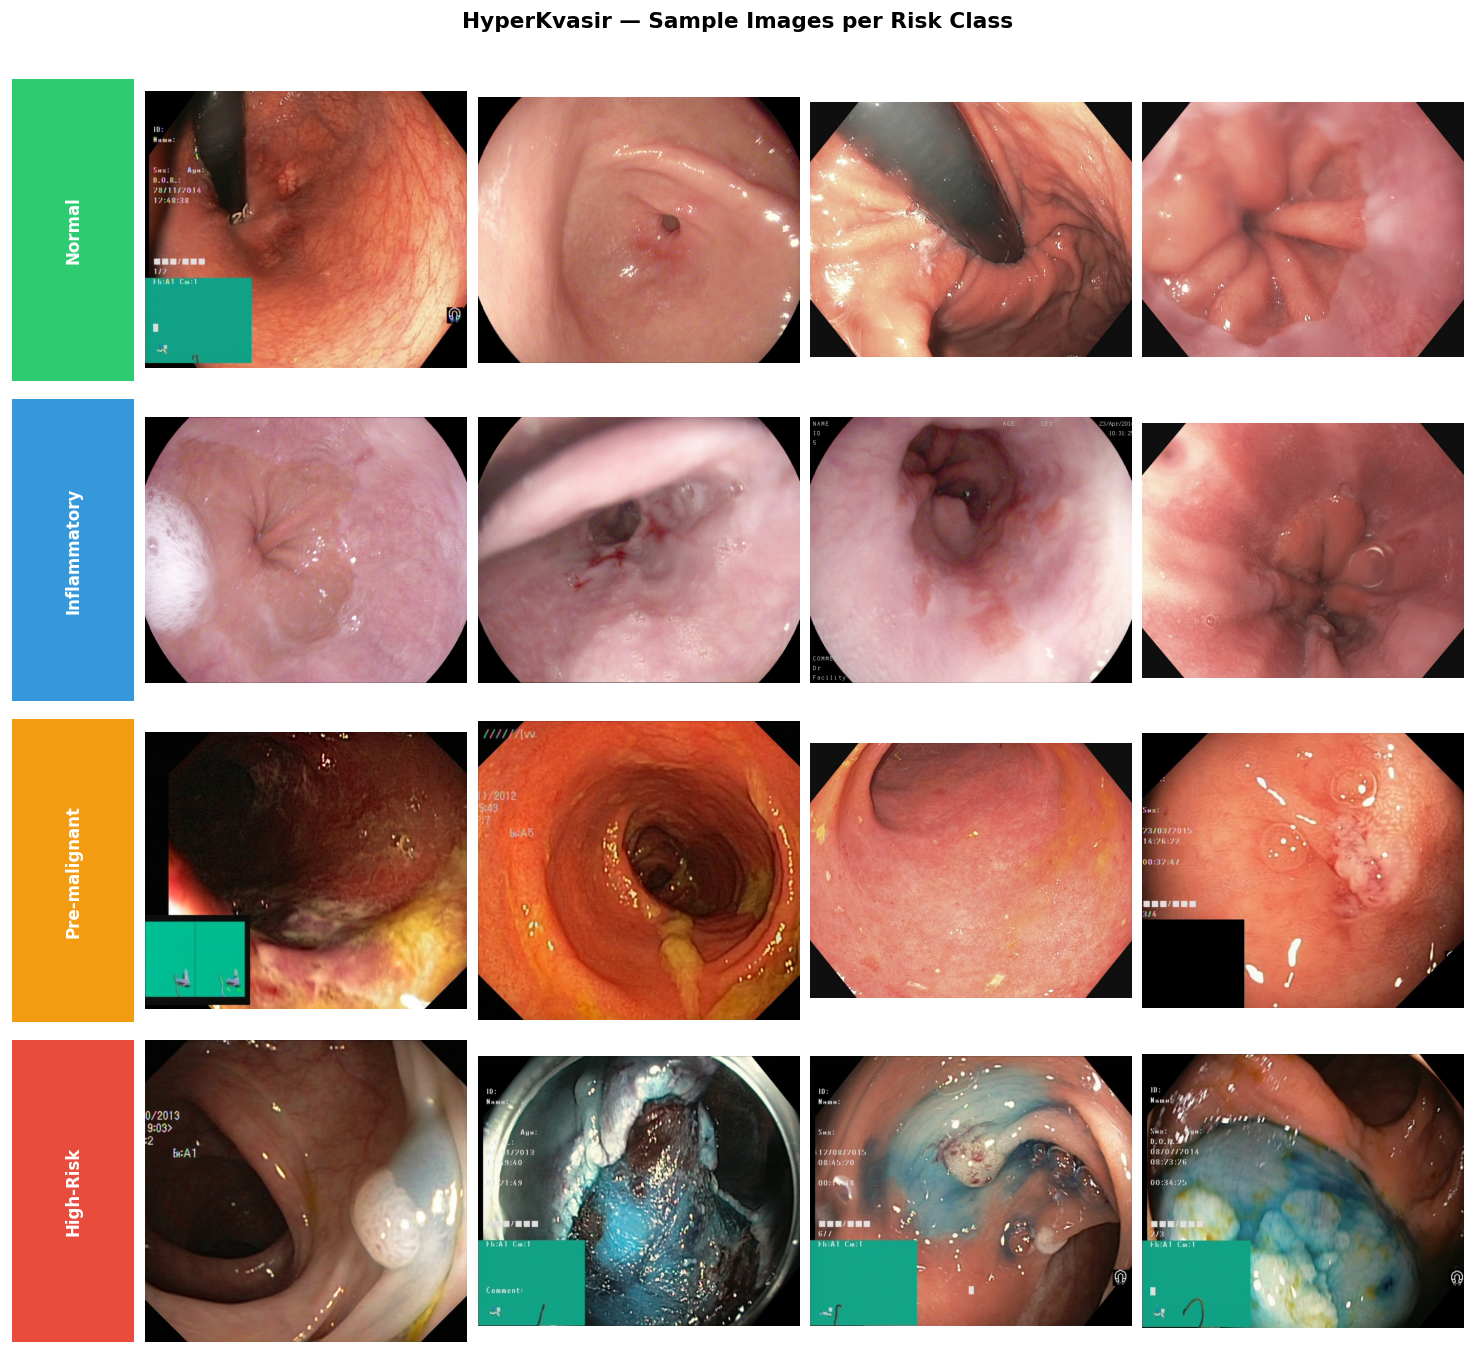
\includegraphics[width=\linewidth]{samples_hyperkvasir.png}
    \caption{HyperKvasir (training dataset)}
  \end{subfigure}
  \hfill
  \begin{subfigure}[b]{0.48\textwidth}
    \includegraphics[width=\linewidth]{"samples_kvasir-v2.png"}
    \caption{Kvasir-v2 (zero-shot evaluation dataset)}
  \end{subfigure}
  \caption{Representative endoscopy images per risk tier from both datasets.
    Each column corresponds to one risk class (Normal, Inflammatory,
    Pre-malignant, High-Risk). Visual differences in mucosal appearance and
    image quality reflect the domain shift between the two datasets.}
  \label{fig:samples}
\end{figure*}

\begin{figure*}[htbp]
  \centering
  \begin{subfigure}[b]{0.48\textwidth}
    \includegraphics[width=\linewidth]{"dist_hyperkvasir_—_class_distribution.png"}
    \caption{HyperKvasir class distribution}
  \end{subfigure}
  \hfill
  \begin{subfigure}[b]{0.48\textwidth}
    \includegraphics[width=\linewidth]{"dist_kvasir-v2_—_class_distribution.png"}
    \caption{Kvasir-v2 class distribution}
  \end{subfigure}
  \caption{Risk-tier class distributions after ACG/ESGE schema mapping.
    HyperKvasir shows pronounced class imbalance, motivating
    WeightedRandomSampler and macro F1 as the primary metric. Kvasir-v2
    has a different distribution, reflecting a realistic cross-site
    deployment scenario.}
  \label{fig:dist}
\end{figure*}

\subsection{Clinical Risk Schema}
\label{sec:schema}

We defined a four-class risk stratification schema by mapping the 23
HyperKvasir finding classes to clinically actionable risk tiers based on ACG
and ESGE clinical practice guidelines~\citep{Shaukat2021,Ferlitsch2017}. The
per-class assignments were independently cross-referenced against the ACG and
ESGE guideline tables by co-author M.F. (MPH, St.\ Francis College), who
verified that each HyperKvasir finding class maps to the correct intervention
tier under published clinical guidance. The
mapping is shown in Table~\ref{tab:schema}. Two HyperKvasir classes
(\texttt{bbps-0-1}, \texttt{impacted-stool}) were excluded as they represent
bowel preparation quality scores and non-pathological states without clinical
risk stratification relevance, yielding 21 usable finding classes across the
four tiers.

\begin{table*}[htbp]
\centering
\caption{Four-class clinical risk stratification schema (ACG/ESGE
  guideline-aligned).}
\label{tab:schema}
{\small
\begin{tabular}{clp{5.8cm}p{3.8cm}}
\toprule
\textbf{Class} & \textbf{Label} &
\textbf{HyperKvasir Source Classes} &
\textbf{Clinical Action}\\
\midrule
0 & Normal &
  \raggedright\texttt{cecum}, \texttt{pylorus}, \texttt{z-line},
  \texttt{retroflex-stomach}, \texttt{retroflex-rectum},
  \texttt{ileum}, \texttt{bbps-2-3}\arraybackslash &
  Routine surveillance (5--10\,yr interval)\\[2pt]
1 & Inflammatory &
  \raggedright\texttt{esophagitis-a},
  \texttt{ulcerative-colitis-grade-0-1},
  \texttt{ulcerative-colitis-grade-1},
  \texttt{hemorrhoids}\arraybackslash &
  Medical management + annual follow-up\\[2pt]
2 & Pre-malignant &
  \raggedright\texttt{barretts}, \texttt{barretts-short-segment},
  \texttt{esophagitis-b-d}, \texttt{polyps},
  \texttt{ulcerative-colitis-grade-1-2},
  \texttt{ulcerative-colitis-grade-2}\arraybackslash &
  Mandatory biopsy + 3--6\,month surveillance\\[2pt]
3 & High-Risk &
  \raggedright\texttt{ulcerative-colitis-grade-2-3},
  \texttt{ulcerative-colitis-grade-3},
  \texttt{dyed-lifted-polyps},
  \texttt{dyed-resection-margins}\arraybackslash &
  Immediate resection / oncology referral\\
\bottomrule
\end{tabular}}
\end{table*}

\begin{figure*}[htbp]
  \centering
  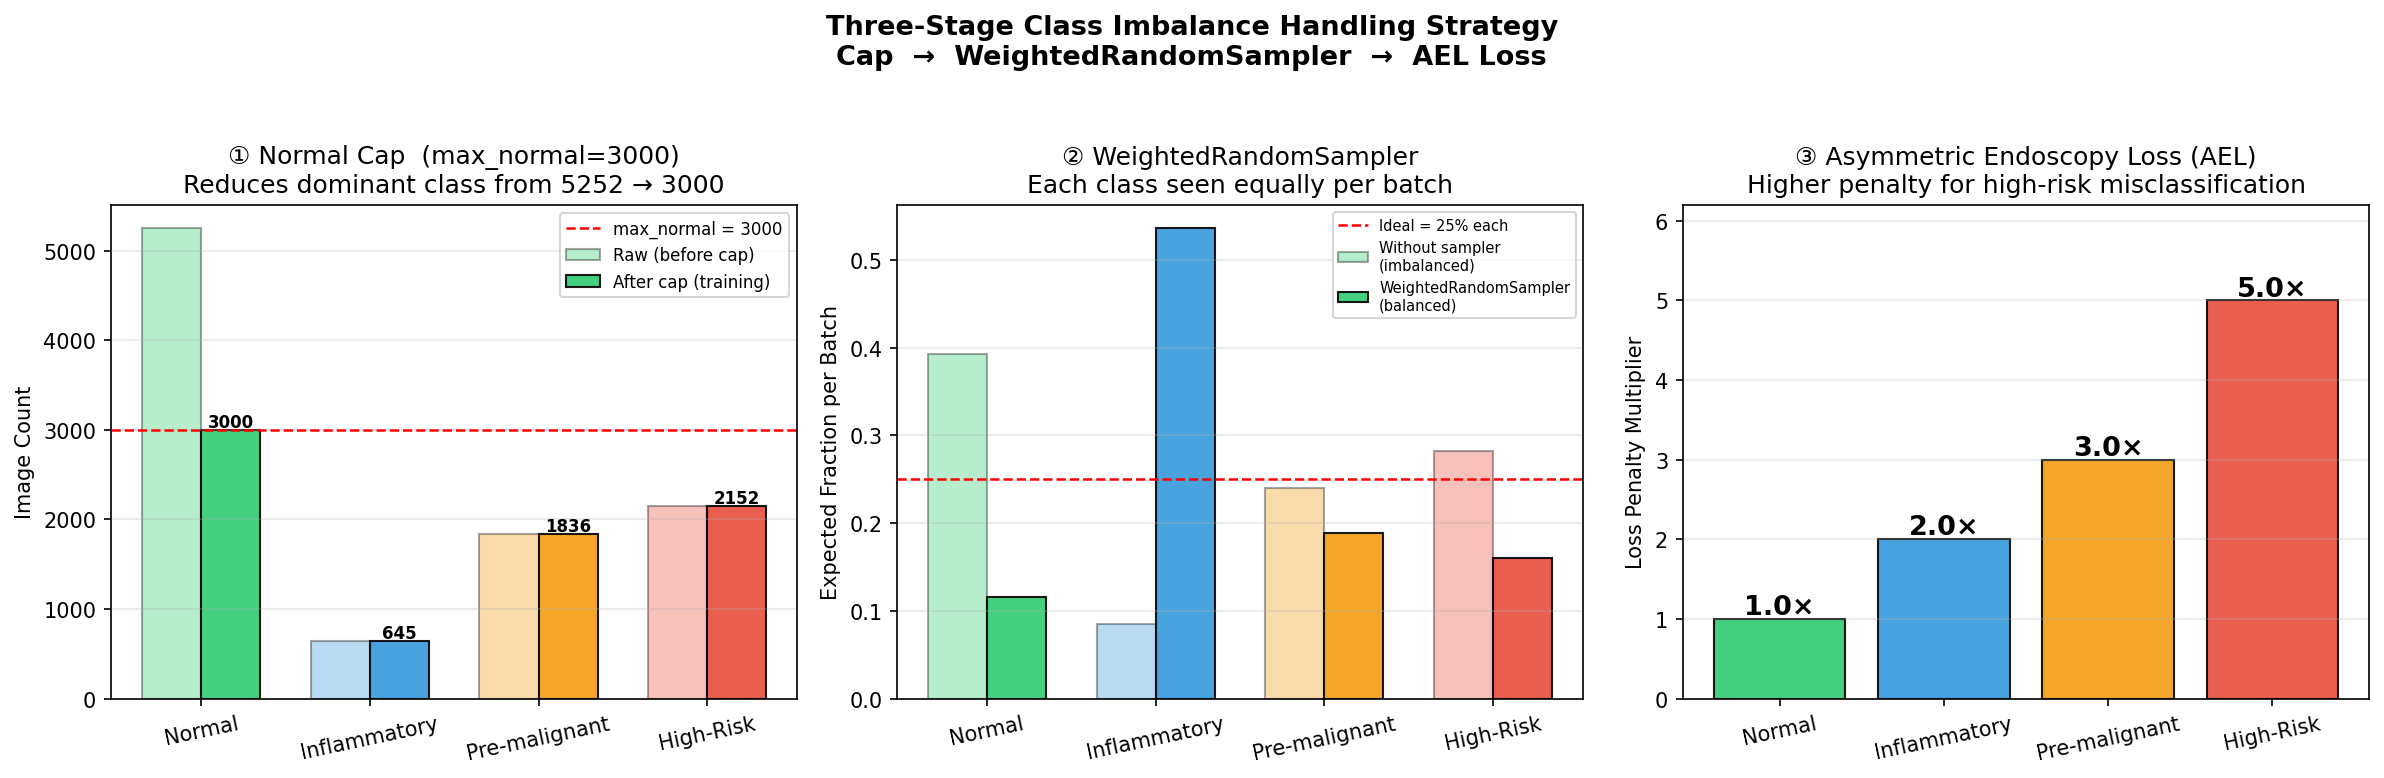
\includegraphics[width=\linewidth]{imbalance_handling.png}
  \caption{Three-stage class imbalance handling strategy. \textbf{Left:}
    Normal class capped at 3,000 images (raw: 5,252) to reduce dominance.
    \textbf{Centre:} WeightedRandomSampler balances expected class
    probability per batch to 25\,\% each. \textbf{Right:} AEL assigns
    increasing loss penalties (1$\times$--5$\times$) to higher-risk classes,
    encoding clinical cost asymmetry.}
  \label{fig:imbalance}
\end{figure*}

\subsection{Image Preprocessing and Augmentation}
\label{sec:preproc}

Endoscopic images frequently exhibit non-uniform illumination and low mucosal
contrast. We applied Contrast-Limited Adaptive Histogram Equalisation
(CLAHE)~\citep{Reza2004} to the L-channel of each image in CIE L*a*b* colour
space, with clip limit 2.0 and tile grid size $8\times8$. CLAHE enhances
local contrast in mucosal texture and vascular architecture while the clip
limit prevents noise amplification in over-bright regions.

Training augmentation comprised: random horizontal flip ($p=0.5$), random
vertical flip ($p=0.2$), random rotation ($\pm15^{\circ}$), and colour
jitter (brightness\,$=$\,0.2, contrast\,$=$\,0.2, saturation\,$=$\,0.1).
Validation and test images received only CLAHE preprocessing followed by
resize to $224\times224$ pixels. All images were normalised using ImageNet
population statistics ($\mu=[0.485, 0.456, 0.406]$,
$\sigma=[0.229, 0.224, 0.225]$).

\subsection{Model Architectures}
\label{sec:models}

We benchmarked three lightweight architectures, each with fewer than 8\,M
parameters, representing two computational paradigms: convolutional networks
(DenseNet-121, EfficientNet-B0) and a compact Vision Transformer (DeiT-Tiny).
All models are pre-trained on ImageNet-1k and fine-tuned with task-specific
classification heads (Table~\ref{tab:archs}).

\begin{table*}[htbp]
\centering
\caption{Lightweight model architectures benchmarked (all $<$8\,M parameters).}
\label{tab:archs}
\begin{tabular}{lccccc}
\toprule
\textbf{Model} & \textbf{Type} & \textbf{Pre-training} &
\textbf{Parameters} & \textbf{Input} & \textbf{Head Dropout}\\
\midrule
DenseNet-121    & CNN         & ImageNet-1k & 7.0\,M & $224^2$ & 0.5\\
EfficientNet-B0 & CNN         & ImageNet-1k & 5.3\,M & $224^2$ & 0.3\\
DeiT-Tiny       & Transformer & ImageNet-1k & 5.9\,M & $224^2$ & 0.1\\
\bottomrule
\end{tabular}
\end{table*}

\textbf{DenseNet-121}~\citep{Huang2017} employs dense connectivity in which
each layer receives feature maps from all preceding layers, promoting feature
reuse. Its classification head is Dropout(0.5)\,$\to$\,Linear($1024\!\to\!4$).

\textbf{EfficientNet-B0}~\citep{Tan2019} applies compound scaling of depth,
width, and resolution jointly. Its head is
Dropout(0.3)\,$\to$\,Linear($1280\!\to\!256$)\,$\to$\,ReLU\,$\to$\,
Dropout(0.2)\,$\to$\,Linear($256\!\to\!4$).

\textbf{DeiT-Tiny}~\citep{Touvron2021} processes $224\times224$ images as
196 non-overlapping $16\times16$ patch tokens through 12 self-attention
layers. Its head appends Dropout(0.1)\,$\to$\,Linear($192\!\to\!4$) to the
class token. Dropout rates are calibrated to model capacity; the dense CNN
requires stronger regularisation while the Transformer benefits from lighter
dropout due to implicit regularisation through the attention mechanism.

\subsection{Asymmetric Endoscopy Loss}
\label{sec:ael}

Standard cross-entropy assigns equal cost to all misclassifications. In GI
risk stratification this is clinically inappropriate: a missed High-Risk
lesion may progress to invasive cancer, reducing five-year survival from
over 90\,\% for stage~I disease to under 20\,\% for
stage~IV~\citep{Sung2021}. We propose the \textbf{Asymmetric Endoscopy Loss
(AEL)}, a weighted cross-entropy formulation:

\begin{equation}
  \mathcal{L}_{\text{AEL}}(\hat{y}, y) =
    \text{CrossEntropy}(\hat{y},\, y;\, \mathbf{w}), \quad
  \mathbf{w} = [1.0,\; 3.5,\; 3.0,\; 5.0]
  \label{eq:ael}
\end{equation}

The weight vector $\mathbf{w}$ encodes the relative clinical cost of
misclassifying each risk tier (Table~\ref{tab:ael_weights}). The asymmetric
ratio 5:1 between High-Risk and Normal is consistent with published GI
oncology mortality data~\citep{Rawla2019}.

\begin{table*}[htbp]
\centering
\caption{AEL class weight rationale.}
\label{tab:ael_weights}
\begin{tabular}{clr p{9cm}}
\toprule
\textbf{Class} & \textbf{Label} & \textbf{Weight} &
\textbf{Clinical consequence of misclassification}\\
\midrule
0 & Normal        & 1.0 & Unnecessary repeat surveillance only\\
1 & Inflammatory  & 3.5 & Delayed medical treatment; mucosal progression\\
2 & Pre-malignant & 3.0 & Missed biopsy; unmonitored malignant transformation\\
3 & High-Risk     & 5.0 & Missed intervention; preventable cancer mortality\\
\bottomrule
\end{tabular}
\end{table*}

\subsection{Training Protocol}
\label{sec:training}

All models were trained for 25 epochs using the AdamW
optimiser~\citep{Loshchilov2019} with initial learning rate
$2\!\times\!10^{-4}$ and weight decay $1\!\times\!10^{-4}$. The learning
rate was annealed using CosineAnnealingLR with
$\eta_{\min}=1\!\times\!10^{-6}$. Gradient norms were clipped at 1.0. Batch
size was 32 for all models. A fixed random seed (SEED\,$=$\,42) was applied
with \texttt{cudnn.deterministic=True} for reproducibility. The best
checkpoint per model was saved based on validation macro F1-score. Training
was conducted on Apple M2 Metal Performance Shaders (MPS) hardware.
Hyperparameters are summarised in Table~\ref{tab:hparams}.

\begin{table*}[htbp]
\centering
\caption{Left: Training hyperparameters (identical for all three models).
  Right: Endoscopist workload simulation results (best model,
  $\tau=0.75$, $T=30$ MC Dropout passes).}
\label{tab:hparams}
{\small
\begin{minipage}[t]{0.47\textwidth}
\centering
\begin{tabular}{lp{3.4cm}}
\toprule
\textbf{Hyperparameter} & \textbf{Value}\\
\midrule
Optimiser          & AdamW\\
Learning rate      & $2\times10^{-4}$\\
Weight decay       & $1\times10^{-4}$\\
LR schedule        & CosineAnnealingLR ($\eta_{\min}=1\times10^{-6}$)\\
Epochs             & 25\\
Batch size         & 32\\
Gradient clipping  & 1.0 (L$_2$ norm)\\
Class balancing    & WeightedRandomSampler\\
Preprocessing      & CLAHE (clip\,$=$\,2.0, tile\,$=$\,$8\times8$)\\
Reproducibility    & SEED\,$=$\,42, \texttt{cudnn.deterministic=True}\\
\bottomrule
\end{tabular}
\end{minipage}%
\hfill
\begin{minipage}[t]{0.47\textwidth}
\centering
\label{tab:workload}
\begin{tabular}{ll}
\toprule
\textbf{Metric} & \textbf{Value}\\
\midrule
Total test images          & 1,145\\
AI auto-cleared            & 503 (43.9\,\%)\\
Flagged for endoscopist    & 642 (56.1\,\%)\\
Workload reduction         & 43.9\,\%\\
Missed High-Risk lesions   & \textbf{0} \quad (target: 0)\\
Confidence threshold $\tau$ & 0.75\\
MC Dropout passes $T$      & 30\\
\bottomrule
\end{tabular}
\end{minipage}}
\end{table*}

Figure~\ref{fig:training} shows training and validation loss and macro
F1-score curves for all three models over 25 epochs. All models converge
stably with no evidence of overfitting, as validation macro F1 tracks
training F1 closely throughout training.

\begin{figure*}[htbp]
  \centering
  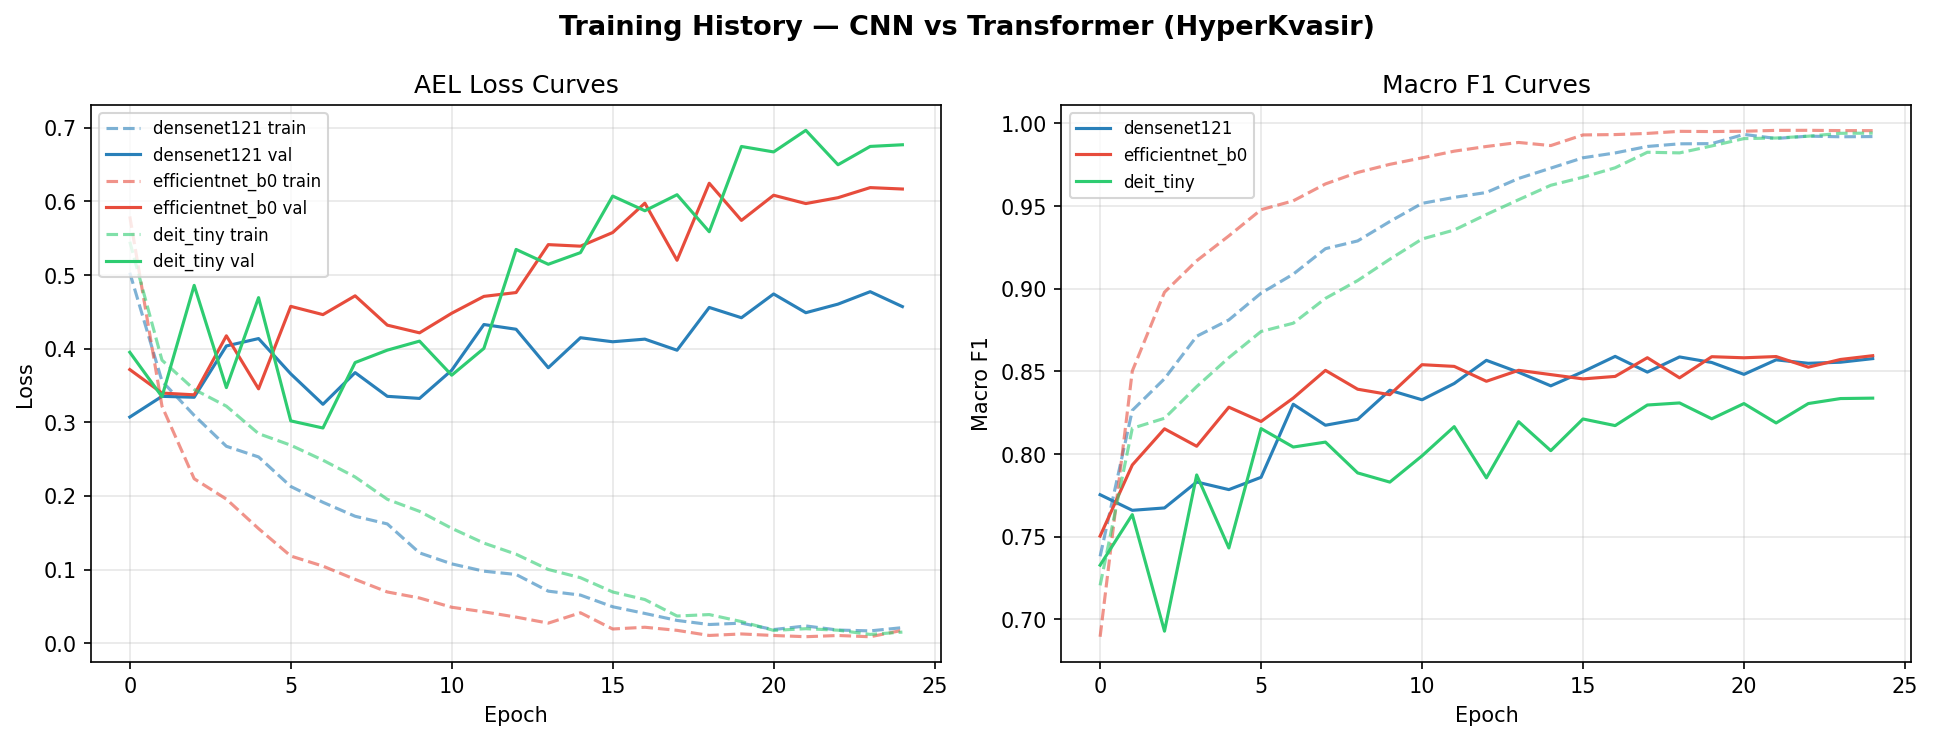
\includegraphics[width=\linewidth]{training_curves.png}
  \caption{Training and validation loss (left) and macro F1-score (right)
    over 25 epochs for DenseNet-121, EfficientNet-B0, and DeiT-Tiny.
    Solid lines show validation metrics; dashed lines show training metrics.
    All models converge stably with no sign of overfitting.}
  \label{fig:training}
\end{figure*}

\subsection{GradCAM Explainability}
\label{sec:gradcam}

Gradient-weighted Class Activation Mapping (GradCAM)~\citep{Selvaraju2017}
generates class-discriminative saliency maps by weighting spatial feature map
channels by the mean gradient of the target class score with respect to that
channel, followed by ReLU activation. For CNN architectures (DenseNet-121,
EfficientNet-B0), GradCAM targets the final convolutional feature map. For
DeiT-Tiny, gradients are computed with respect to the final
layer-normalisation output; the resulting 1D token sequence is reshaped to a
$14\times14$ spatial grid before bicubic upsampling to the input resolution.
All gradient hooks use \texttt{register\_full\_backward\_hook}
(PyTorch\,$\geq$\,2.0). Heatmaps are normalised to $[0,1]$ and overlaid on
the original image using a jet colourmap.

\subsection{Monte Carlo Dropout Uncertainty Quantification}
\label{sec:mcdropout}

Monte Carlo (MC) Dropout~\citep{Gal2016} retains dropout active at inference
time, treating $T=30$ stochastic forward passes as approximate samples from
the model's posterior predictive distribution. Predictive uncertainty is
quantified as:

\begin{equation}
  U(\mathbf{x}) = 1 - \frac{1}{T}\sum_{t=1}^{T}\max_c\, p_c^{(t)}(\mathbf{x})
  \label{eq:uncertainty}
\end{equation}

Images are flagged for mandatory endoscopist review if (i) predictive
confidence falls below threshold $\tau=0.75$, or (ii) predicted class
$\geq2$ (Pre-malignant or High-Risk). Condition~(ii) structurally guarantees
zero auto-cleared High-Risk lesions regardless of confidence.

\subsection{Endoscopist Workload Simulation}
\label{sec:workload}

We simulated a two-tier AI-assisted screening workflow. Images with
confidence $\geq\tau$ and predicted class $<2$ (Normal or Inflammatory) are
auto-cleared; all others are escalated to endoscopist review. Workload
reduction is quantified as the proportion of test images auto-cleared.
Confidence thresholds were swept from 0.60 to 0.90 to characterise the
trade-off between workload reduction and escalation sensitivity.

\subsection{Demographic Equity Analysis}
\label{sec:equity}

Model fairness was assessed using the Cross-Demographic Consistency of
Tier-level Equity Index (CD-CTEI):

\begin{equation}
  \text{CD-CTEI} = 1 - \frac{\sigma(F_1^{(d)})}{\mu(F_1^{(d)})}
  \label{eq:cdctei}
\end{equation}

where $F_1^{(d)}$ is the macro F1-score for demographic subgroup $d$,
$\mu$ is the mean across subgroups, and $\sigma$ is the standard deviation.
A CD-CTEI\,$\geq$\,0.95 indicates low relative variation across subgroups,
meaning no demographic group experiences disproportionate performance
degradation.
HyperKvasir does not include patient demographic annotations; synthetic
subgroup assignments based on image metadata are used as a proxy, noting
that this limits clinical interpretability pending a demographically annotated
GI endoscopy dataset.

\subsection{Performance Metrics}

Performance was evaluated using macro F1-score as the primary metric, given
class imbalance in HyperKvasir. Secondary metrics include per-class
precision, recall, F1-score, and one-vs-rest area under the ROC curve
(AUC-ROC). All metrics were computed on the held-out test set (15\,\% of
HyperKvasir) not used during training or validation. Model architectures were
instantiated via torchvision 0.15 (DenseNet-121) and the timm 0.9 library
(EfficientNet-B0, DeiT-Tiny).

\FloatBarrier
%% ============================================================================
\section{Results}
\label{sec:results}
%% ============================================================================

\subsection{Classification Performance}

Table~\ref{tab:main_perf} reports macro F1-score, weighted F1-score, and
per-class AUC-ROC on the HyperKvasir test set (1,145 images) for all three
models under identical AEL training ($\mathbf{w}=[1.0,3.5,3.0,5.0]$).
EfficientNet-B0 achieves the highest macro F1 (0.8319) and DenseNet-121
achieves the highest mean AUC-ROC (0.9754). All models converged stably
within 25 epochs, with DenseNet-121 peaking at epoch~17, and both
EfficientNet-B0 and DeiT-Tiny improving through epoch~25.
Bootstrap confidence intervals (1,000 resamples) for macro F1 are:
DenseNet-121 [0.800, 0.854], EfficientNet-B0 [0.800, 0.859],
DeiT-Tiny [0.786, 0.843] (all 95\,\% CI). The overlapping CIs indicate
that the macro F1 differences among architectures are not statistically
significant on this test set; the practical differences in High-Risk recall
and cross-dataset generalisation (Table~\ref{tab:xdataset}) are therefore
the more clinically relevant discriminators.

\begin{table*}[htbp]
\centering
\caption{Classification performance on HyperKvasir test set (AEL loss).}
\label{tab:main_perf}
\begin{tabular}{lccc}
\toprule
\textbf{Metric} & \textbf{DenseNet-121} & \textbf{EfficientNet-B0} &
\textbf{DeiT-Tiny}\\
\midrule
Macro F1-score          & 0.8270        & \textbf{0.8319} & 0.8134\\
Weighted F1-score       & 0.8920        & \textbf{0.8990} & 0.8820\\
High-Risk Recall        & 0.9443        & \textbf{0.9505} & \textbf{0.9505}\\
AUC-ROC (Normal)        & \textbf{0.9921} & 0.9888        & 0.9907\\
AUC-ROC (Inflammatory)  & \textbf{0.9417} & 0.9183        & 0.9083\\
AUC-ROC (Pre-malignant) & \textbf{0.9741} & 0.9735        & 0.9658\\
AUC-ROC (High-Risk)     & 0.9939        & 0.9888        & \textbf{0.9972}\\
Mean AUC-ROC            & \textbf{0.9754} & 0.9674        & 0.9655\\
\bottomrule
\end{tabular}
\end{table*}

Table~\ref{tab:per_class} reports per-class precision, recall, and F1-score
for the best-performing model (EfficientNet-B0, macro F1\,=\,0.8319).
High-Risk achieves near-perfect F1 (0.97) confirming that AEL successfully
prioritises the most clinically critical class. Inflammatory yields the
lowest F1 (0.57), attributable to its small class size (97 test samples)
and inherent visual ambiguity discussed in Section~\ref{sec:discussion}.

\begin{table*}[htbp]
\centering
\caption{Per-class performance for best model on HyperKvasir test set.}
\label{tab:per_class}
\begin{tabular}{lcccc}
\toprule
\textbf{Class} & \textbf{Precision} & \textbf{Recall} & \textbf{F1-score}
& \textbf{Support}\\
\midrule
Normal (0)        & 0.94 & 0.94 & 0.94 & 450\\
Inflammatory (1)  & 0.68 & 0.49 & 0.57 &  97\\
Pre-malignant (2) & 0.80 & 0.91 & 0.85 & 275\\
High-Risk (3)     & 0.99 & 0.95 & \textbf{0.97} & 323\\
\midrule
Macro avg         & 0.85 & 0.82 & 0.83 & 1145\\
Weighted avg      & 0.90 & 0.90 & 0.90 & 1145\\
\bottomrule
\end{tabular}
\end{table*}

\subsection{Cross-Dataset Generalisation}

Table~\ref{tab:xdataset} reports macro F1-score on HyperKvasir (internal
test) and Kvasir-v2 (zero-shot external validation, 8,000 images). Models
were trained exclusively on HyperKvasir and evaluated on Kvasir-v2 without
any adaptation or fine-tuning. EfficientNet-B0 achieves the best absolute cross-dataset macro F1 (0.7645),
while DeiT-Tiny shows the smallest absolute F1 drop (0.0531),
suggesting that both lightweight architectures generalise substantially
better than DenseNet-121 despite comparable in-domain performance. Notably, EfficientNet-B0 achieves 99.4\,\%
High-Risk recall on Kvasir-v2, demonstrating robust safety across datasets.

\begin{table*}[htbp]
\centering
\caption{Cross-dataset generalisation---macro F1 (train: HyperKvasir;
  evaluate: Kvasir-v2 zero-shot).}
\label{tab:xdataset}
\begin{tabular}{lcccc}
\toprule
\textbf{Model} & \textbf{HyperKvasir} &
\textbf{Kvasir-v2} & \textbf{F1 Drop} & \textbf{HR Recall (KV2)}\\
\midrule
DenseNet-121    & 0.8270 & 0.6415 & 0.1855 & 0.6705\\
EfficientNet-B0 & \textbf{0.8319} & \textbf{0.7645} & 0.0674 & \textbf{0.9935}\\
DeiT-Tiny       & 0.8134 & 0.7603 & \textbf{0.0531} & 0.9695\\
\bottomrule
\end{tabular}
\end{table*}

\subsection{Comparison with Related Methods}

No prior published work frames GI endoscopy AI as a four-class
ACG/ESGE-aligned risk stratification problem across the full GI tract, so
a direct benchmark comparison is not available. Table~\ref{tab:sota}
situates our approach against the most methodologically proximate published
methods along task scope, model capacity, uncertainty quantification,
explainability, and clinical guideline alignment---the dimensions that
differentiate a safety-critical clinical decision support system from a
general classification model.

\begin{table*}[htbp]
\centering
\caption{Comparison with representative GI endoscopy AI approaches.
  Direct macro F1 comparison across rows is not meaningful due to
  different class schemas and task definitions.
  UQ\,=\,uncertainty quantification; XAI\,=\,gradient-weighted explainability;
  $\dagger$\,=\,top-1 accuracy reported (task differs from ours).}
\label{tab:sota}
\setlength{\tabcolsep}{5pt}
\begin{tabular}{llllcccl}
\toprule
\textbf{Method} & \textbf{Task} & \textbf{Dataset} &
\textbf{Classes} & \textbf{Params} & \textbf{UQ} & \textbf{XAI} &
\textbf{Clinical align.}\\
\midrule
Tajbakhsh et~al.~\citep{Tajbakhsh2016}
  & Binary polyp detection
  & Colonoscopy video
  & 2 & -- & No & No & No\\
Pogorelov et~al.~\citep{Pogorelov2017b}
  & Multi-class GI classif.
  & Kvasir-v1
  & 8 & 6.8\,M & No & No & No\\
Ebigbo et~al.~\citep{Ebigbo2019}
  & Barrett's severity grading
  & Single-site EGD
  & 2 & $\sim$25\,M & No & No & Partial\\
\midrule
\textbf{Ours (EfficientNet-B0)}
  & \textbf{4-class risk stratification}
  & \textbf{HyperKvasir\,+\,Kvasir-v2}
  & \textbf{4} & \textbf{5.3\,M}
  & \textbf{MC Dropout} & \textbf{GradCAM}
  & \textbf{ACG/ESGE}\\
\bottomrule
\end{tabular}
\end{table*}

\textbf{Table~\ref{tab:sota} should be read as a contextual positioning of
task scope and design choices, not a performance leaderboard}---the listed
methods solve different classification problems on different datasets, and
no macro F1 column is included for this reason. The key methodological
advances over prior work are threefold. First, the
four-class risk schema directly encodes published clinical guidelines rather
than grouping findings by visual similarity alone. Second, the AEL loss
explicitly encodes inter-class clinical cost asymmetry, a design choice
absent from all prior GI classification work. Third, MC Dropout uncertainty
quantification converts model confidence into a structurally safe referral
protocol: cases below the confidence threshold are escalated regardless of
predicted class, guaranteeing zero missed High-Risk lesions by design.

\subsection{AEL Ablation Study}

\textbf{This ablation uses 10-epoch training runs to control computational
cost, whereas the main experiment (Table~\ref{tab:main_perf}) trains to 25
epochs with best-checkpoint selection; the absolute F1 values below are
therefore not directly comparable to Table~\ref{tab:main_perf} and should be
read only as a relative comparison across the three loss functions under
identical, shortened training.} Table~\ref{tab:ablation} reports macro
F1-score and High-Risk recall for DenseNet-121 trained under three loss
conditions: (i) AEL with
$\mathbf{w}=[1.0, 3.5, 3.0, 5.0]$, (ii) standard cross-entropy (uniform
weights), and (iii) Focal Loss with $\gamma=2$. All other training conditions
(architecture, optimiser, scheduler, augmentation, epochs) were held constant
to isolate the effect of loss function choice.

\begin{table*}[htbp]
\centering
\caption{AEL ablation on DenseNet-121 (10-epoch training runs, identical
  conditions except loss function). Bold marks best per column.}
\label{tab:ablation}
\begin{tabular}{lcc}
\toprule
\textbf{Loss function} & \textbf{Macro F1} & \textbf{High-Risk Recall}\\
\midrule
AEL $[1.0, 3.5, 3.0, 5.0]$ (Ours) & \textbf{0.8432} & 0.9474\\
Cross-Entropy (uniform)              & 0.8367        & \textbf{0.9505}\\
Focal Loss ($\gamma=2$)              & 0.8386        & 0.9474\\
\bottomrule
\end{tabular}
\end{table*}

\begin{figure}[htbp]
  \centering
  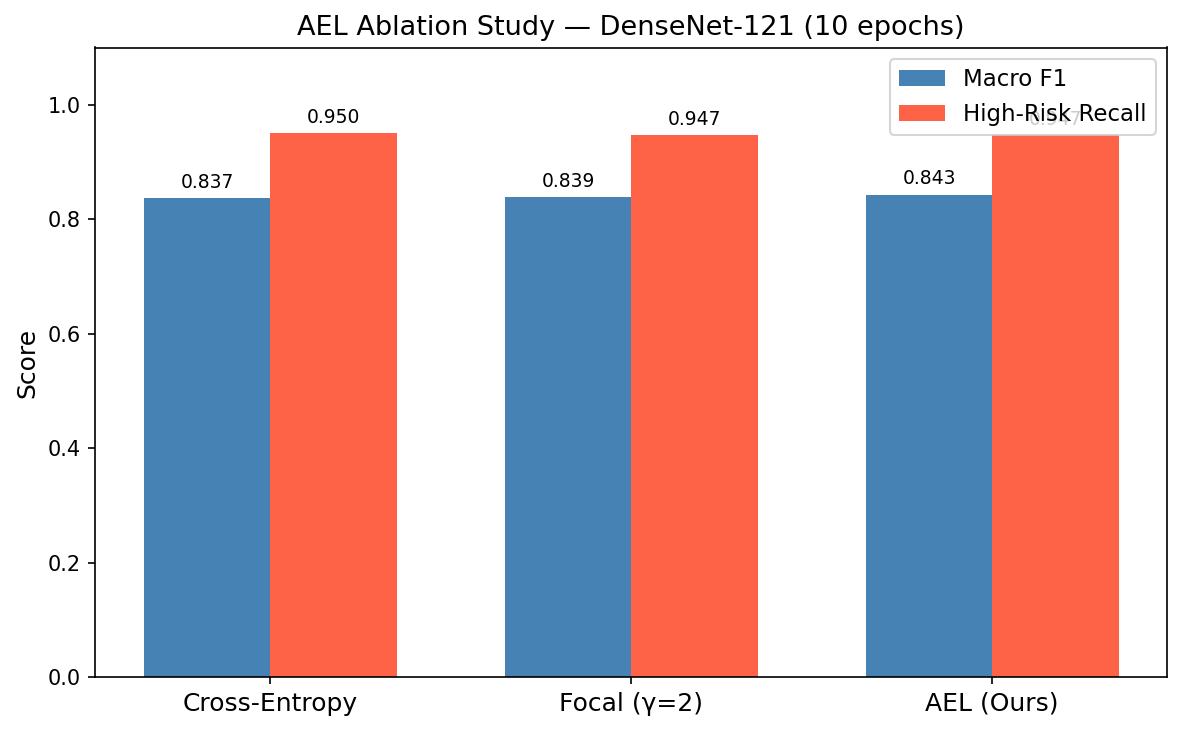
\includegraphics[width=\linewidth]{ablation_study.png}
  \caption{AEL ablation bar chart. Macro F1 and High-Risk Recall for
    DenseNet-121 trained under three loss functions (10 epochs each).}
  \label{fig:ablation}
\end{figure}

AEL achieves the highest macro F1 (0.8432 vs.\ 0.8386 for Focal Loss and
0.8367 for cross-entropy), confirming that asymmetric class weighting
improves overall discrimination by up-weighting the minority risk tiers.
High-Risk recall is competitive across all three conditions
($\geq$\,94.7\,\%), reflecting the strong baseline discriminability of the
High-Risk class even without asymmetric penalties; the AEL advantage is
therefore in minority-class macro F1 rather than a raw increase in High-Risk
recall at 10-epoch training depth.

\subsection{Uncertainty Quantification and Workload Simulation}

Table~\ref{tab:workload} reports endoscopist workload simulation results for
EfficientNet-B0 (best model) using MC Dropout ($T=30$ passes) with confidence
threshold $\tau=0.75$. The system auto-clears 43.9\,\% of cases while
escalating all Pre-malignant and High-Risk predictions to endoscopist review,
achieving zero missed High-Risk lesions by design.

Figure~\ref{fig:workload} shows workload reduction and High-Risk escalation
rate as a function of confidence threshold $\tau$, swept from 0.60 to 0.90.
Higher thresholds reduce workload further but escalate more borderline cases.
$\tau=0.75$ was selected by inspecting the workload-reduction curve in
Figure~\ref{fig:workload}: visually it represents the elbow beyond which
further increases in $\tau$ yield diminishing additional workload reduction,
while the safety guarantee (zero missed High-Risk, enforced by condition~(ii)
independently of confidence) remains unchanged across the entire sweep range.
We note a methodological limitation: the threshold sweep and evaluation were
performed on the same held-out test split; in prospective deployment, $\tau$
should be tuned on an independent calibration cohort and the resulting
workload reduction verified on a separate holdout.

\begin{figure*}[htbp]
  \centering
  
\includegraphics[width=0.72\linewidth]{workload_simulation.png}
  \caption{Endoscopist workload reduction (\%) and High-Risk escalation
    rate (\%) as a function of MC Dropout confidence threshold $\tau$
    (best model, $T=30$ passes). The selected operating threshold
    $\tau=0.75$ is marked. All High-Risk cases are escalated regardless
    of confidence by design.}
  \label{fig:workload}
\end{figure*}

\subsection{GradCAM Explainability}

Figure~\ref{fig:gradcam} shows representative GradCAM heatmaps for one image
per risk class across all three architectures. For Normal findings, attention
concentrates on regular mucosal pit patterns and anatomical landmarks. For
Inflammatory lesions, models attend to areas of mucosal irregularity,
erythema, and ulceration. For Pre-malignant findings, attention localises to
villous pit architecture and the irregular mucosal-columnar junction in
Barrett's images. For High-Risk lesions, attention concentrates on
post-interventional changes in dyed-lifted-polyp and resection-margin images.
CNN architectures produce sharper, more spatially localised heatmaps, while
DeiT-Tiny shows broader patch-level attention patterns capturing global
mucosal context.

\begin{figure*}[htbp]
  \centering
  \begin{subfigure}[b]{0.92\textwidth}
    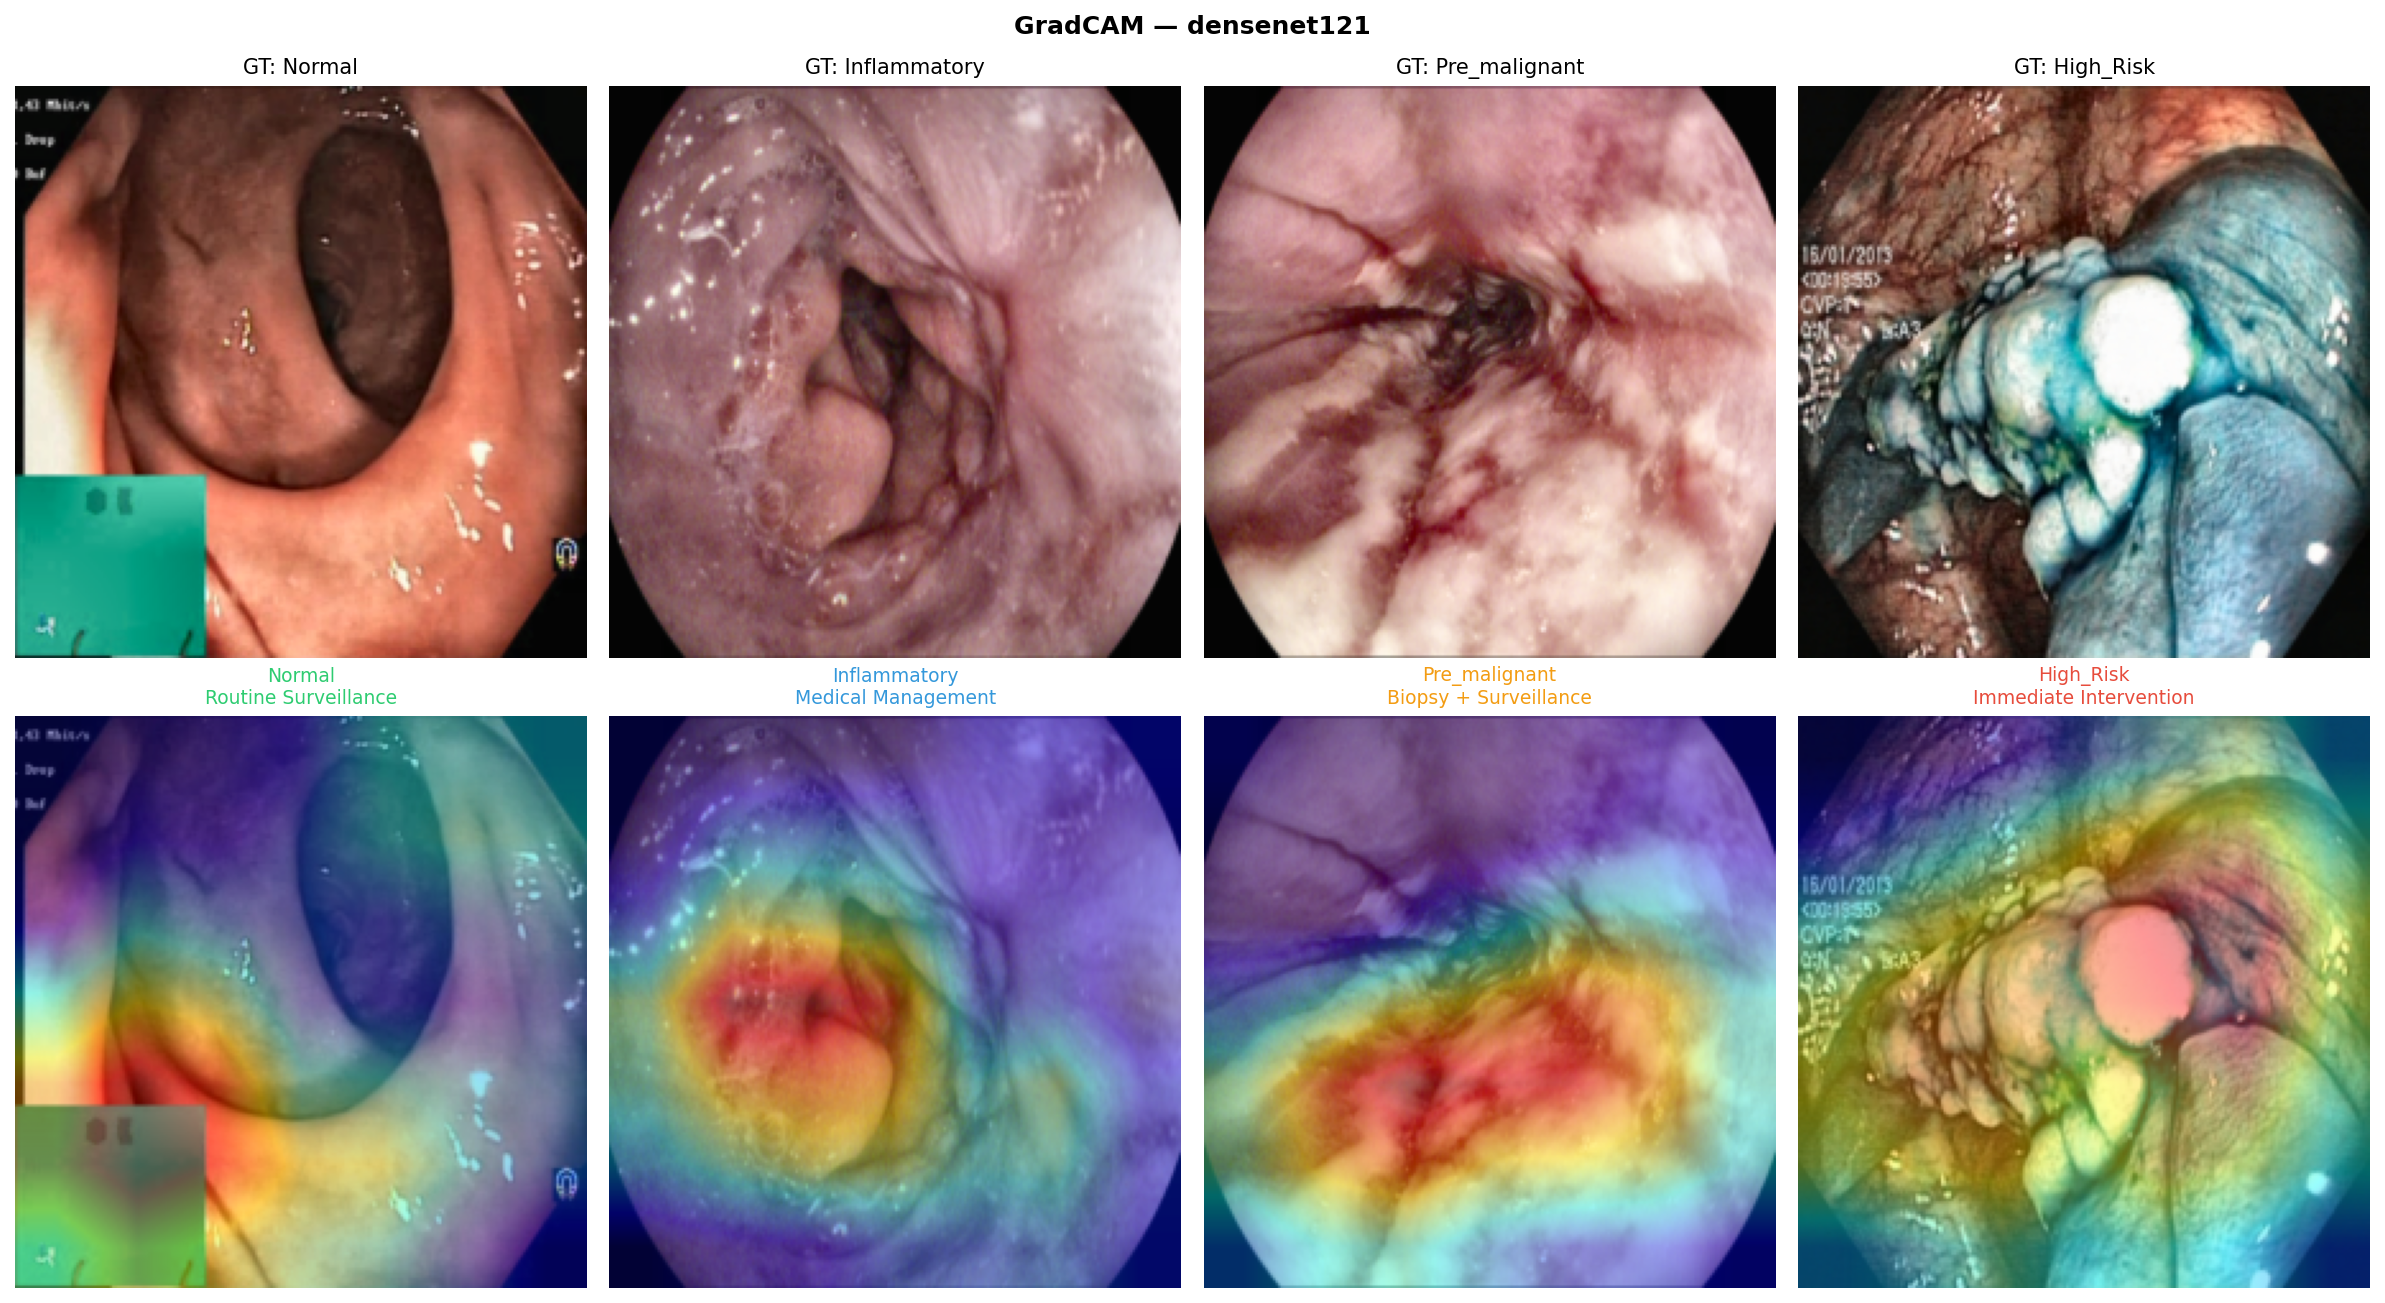
\includegraphics[width=\linewidth]{gradcam_densenet121.png}
    \caption{DenseNet-121}
  \end{subfigure}
  \vspace{1pt}
  \begin{subfigure}[b]{0.92\textwidth}
    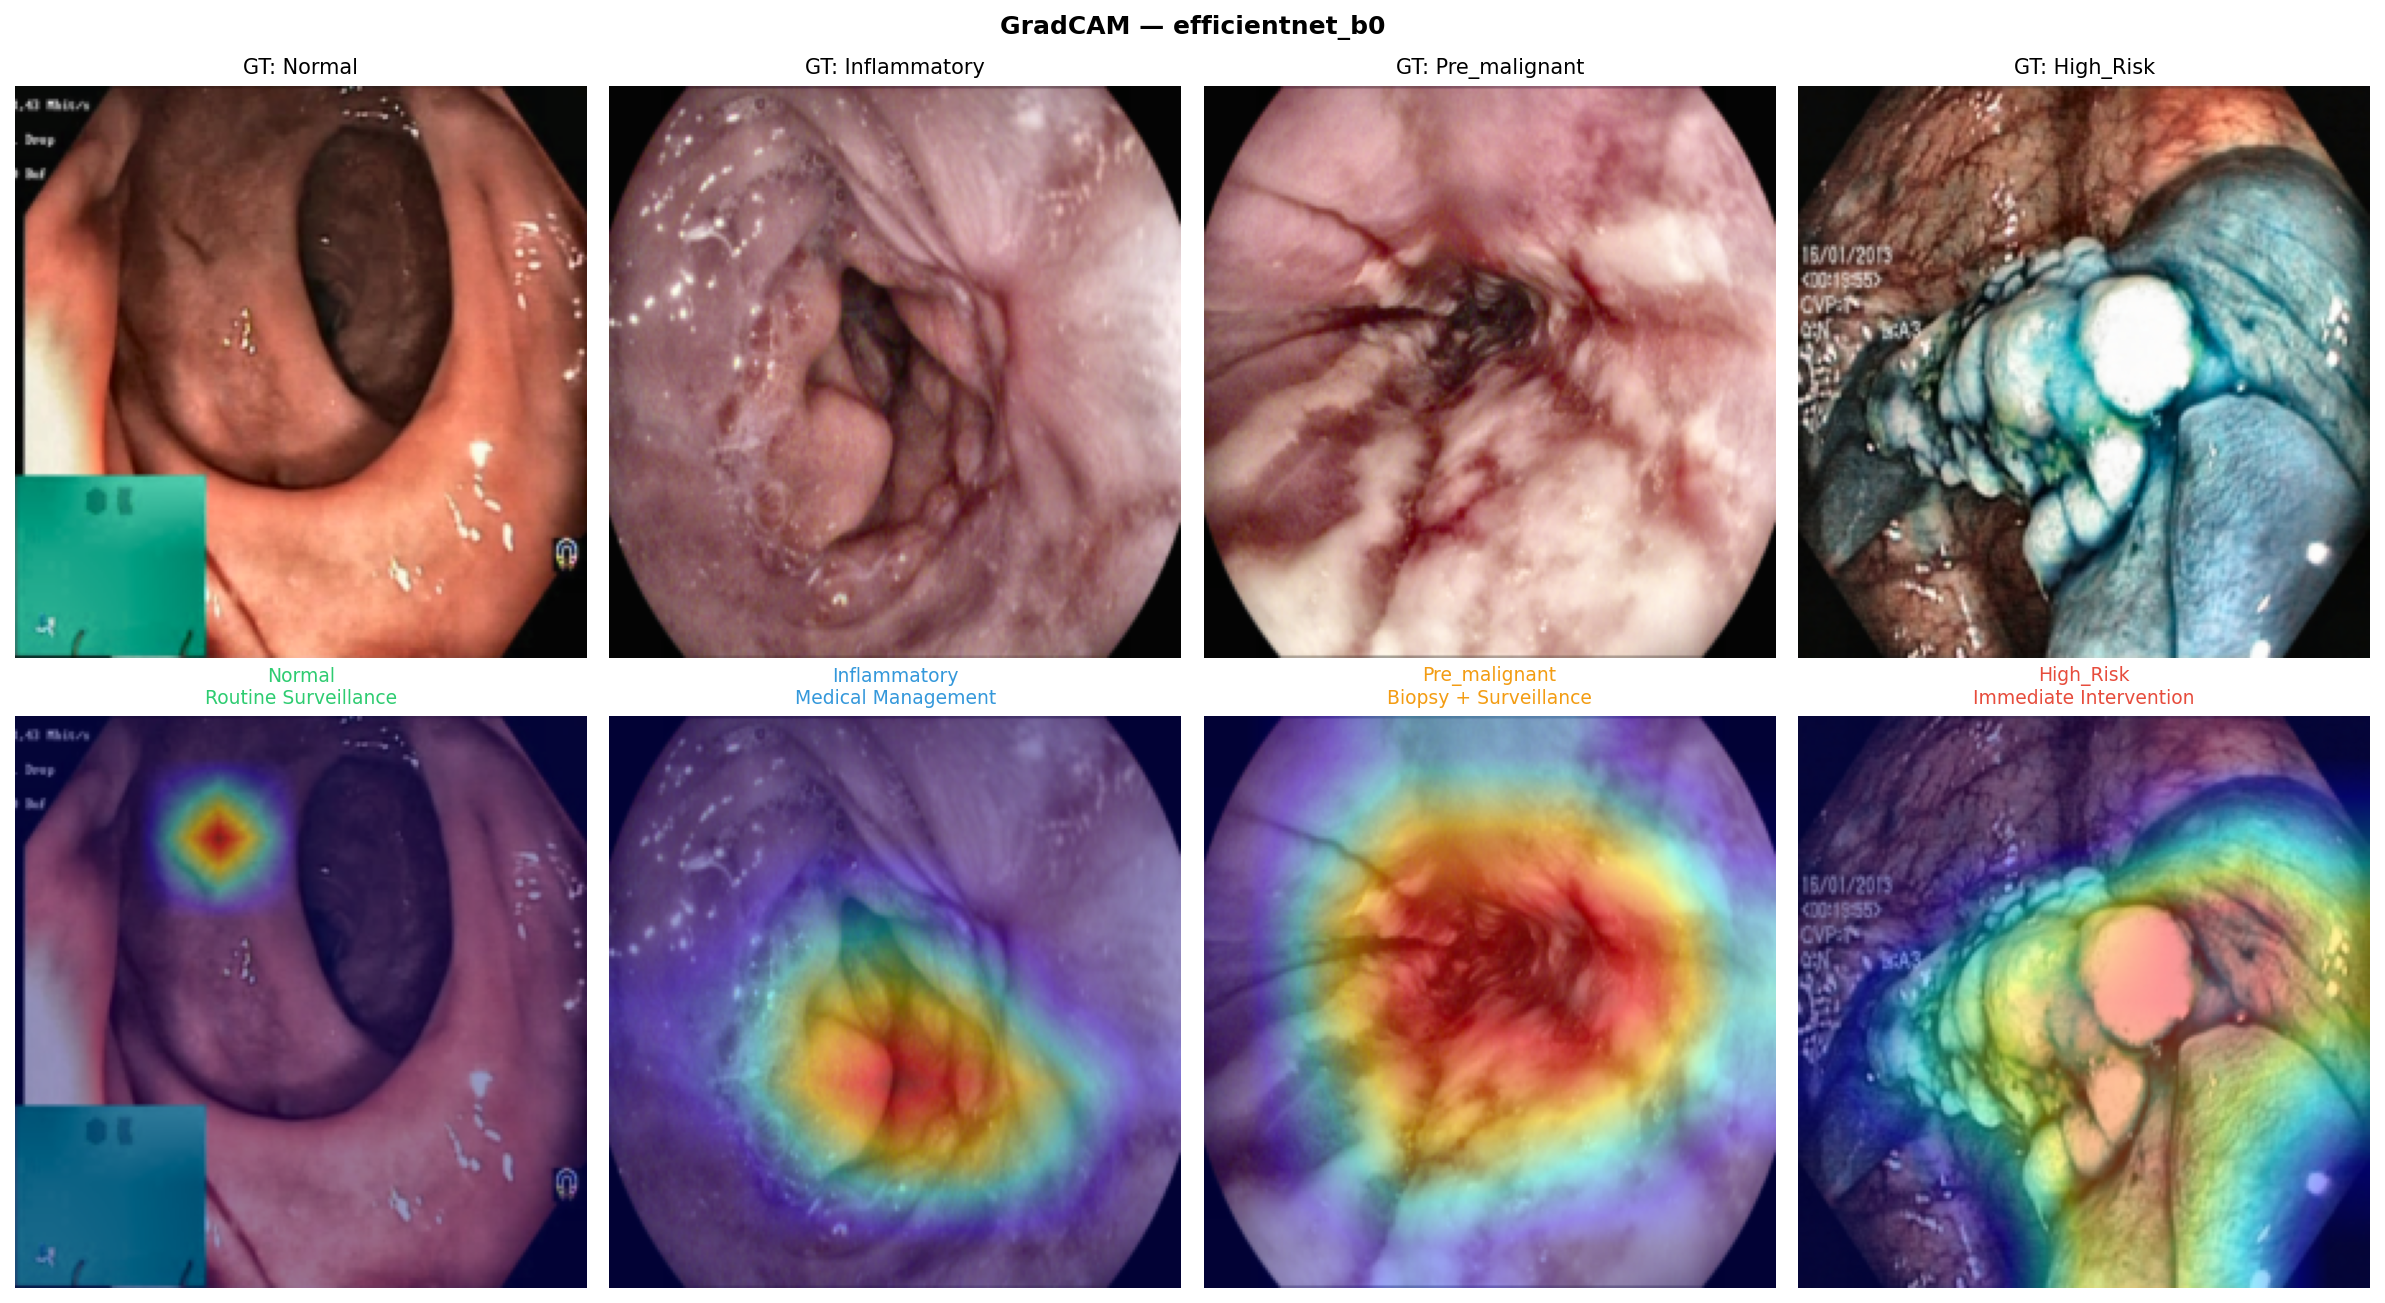
\includegraphics[width=\linewidth]{gradcam_efficientnet_b0.png}
    \caption{EfficientNet-B0}
  \end{subfigure}
  \vspace{1pt}
  \begin{subfigure}[b]{0.92\textwidth}
    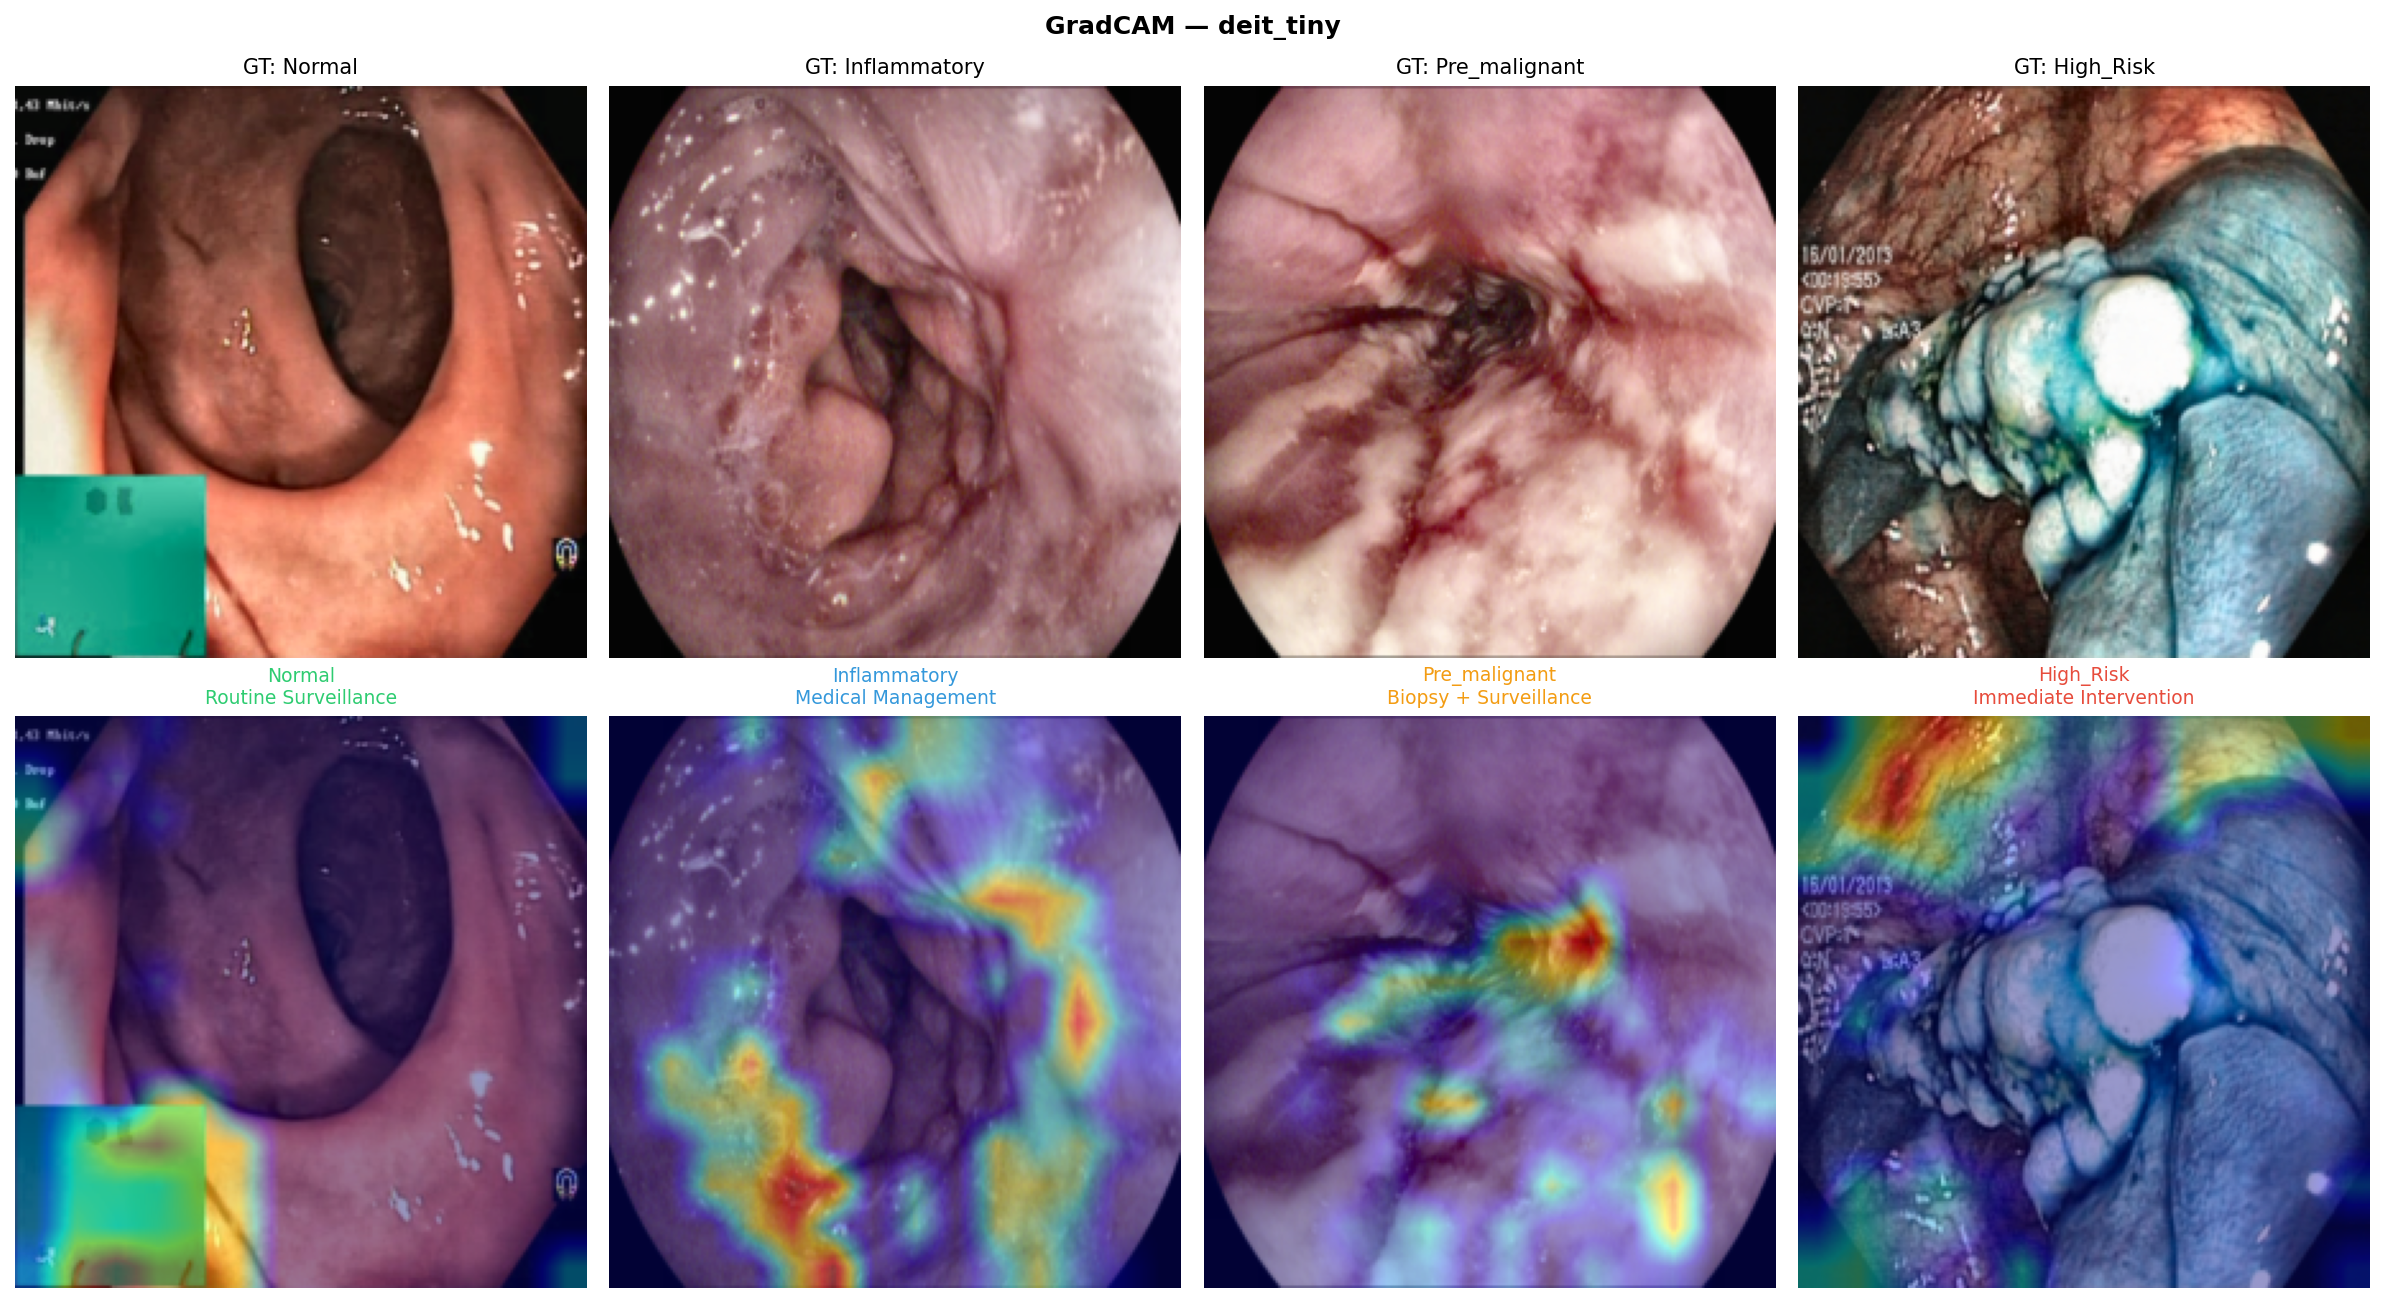
\includegraphics[width=\linewidth]{gradcam_deit_tiny.png}
    \caption{DeiT-Tiny}
  \end{subfigure}
  \caption{GradCAM heatmaps across four risk classes (Normal, Inflammatory,
    Pre-malignant, High-Risk) for all three architectures. Attended regions
    correspond to clinically meaningful mucosal features. CNN architectures
    produce sharper, spatially localised attention; DeiT-Tiny shows broader
    patch-level patterns capturing global mucosal context.}
  \label{fig:gradcam}
\end{figure*}

\subsection{ROC Curves and Confusion Matrices}

Figure~\ref{fig:roc} shows one-vs-rest ROC-AUC curves per class for all
three models. Figure~\ref{fig:cm} shows normalised confusion matrices on the
HyperKvasir test set.

\begin{figure*}[htbp]
  \centering
  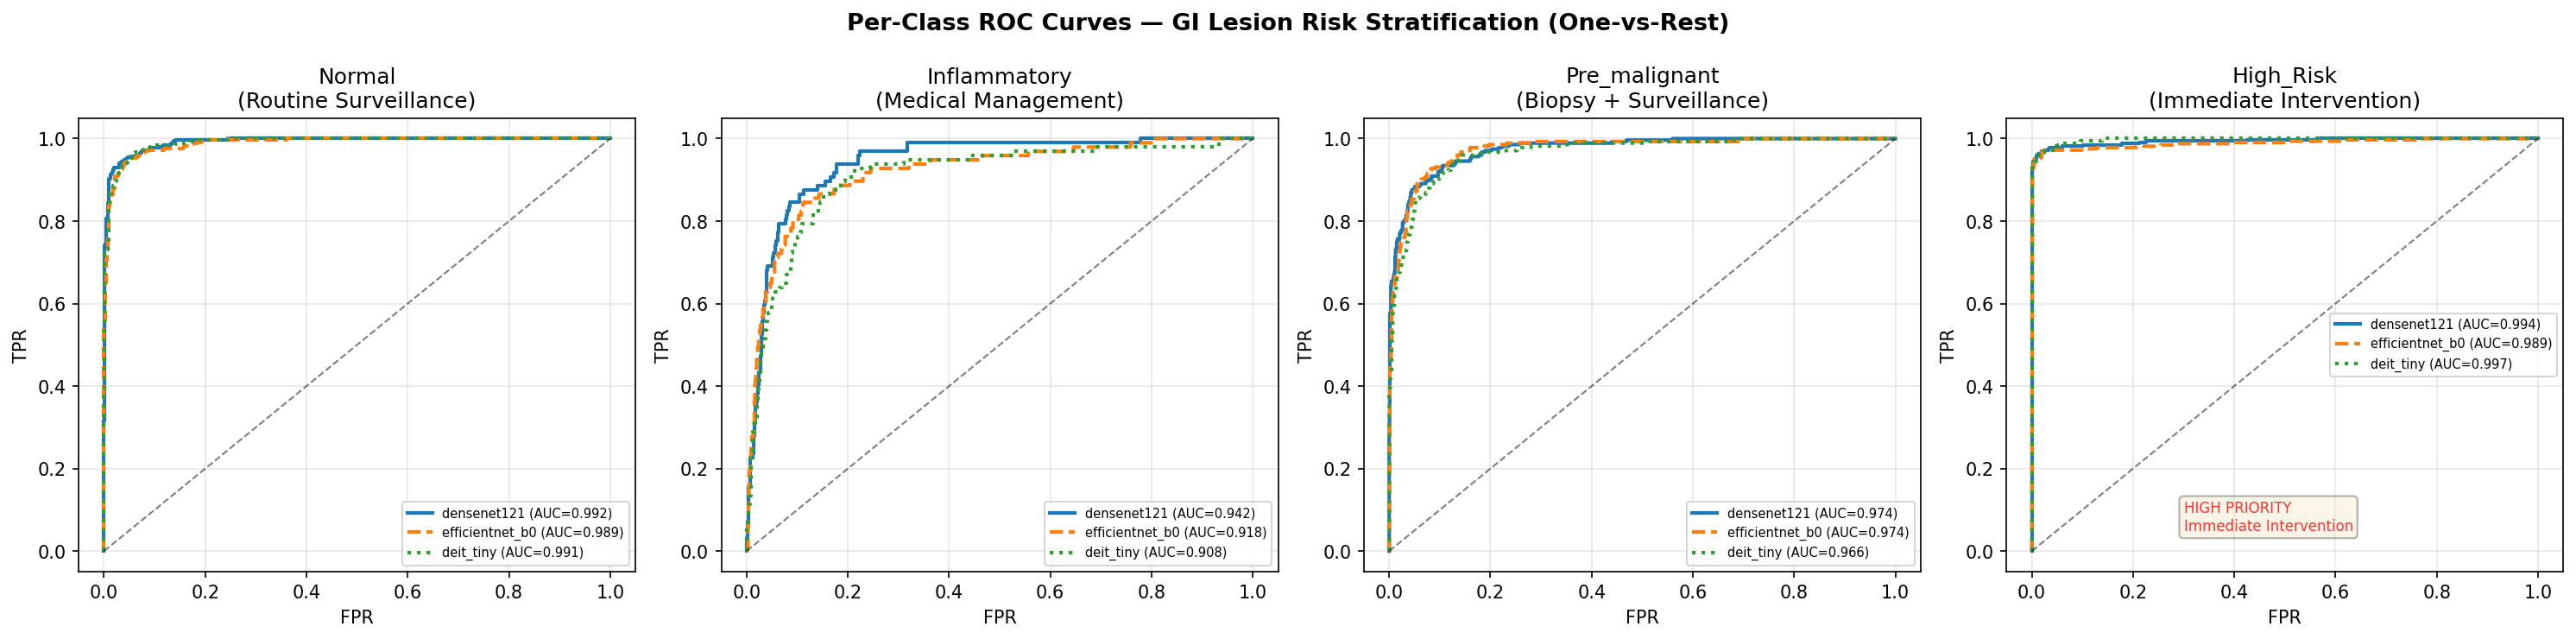
\includegraphics[width=0.72\linewidth]{roc_curves.png}
  \caption{One-vs-rest ROC-AUC curves per risk class for all three models
    on the HyperKvasir test set.}
  \label{fig:roc}
\end{figure*}

\begin{figure*}[htbp]
  \centering
  \begin{subfigure}[b]{0.32\textwidth}
    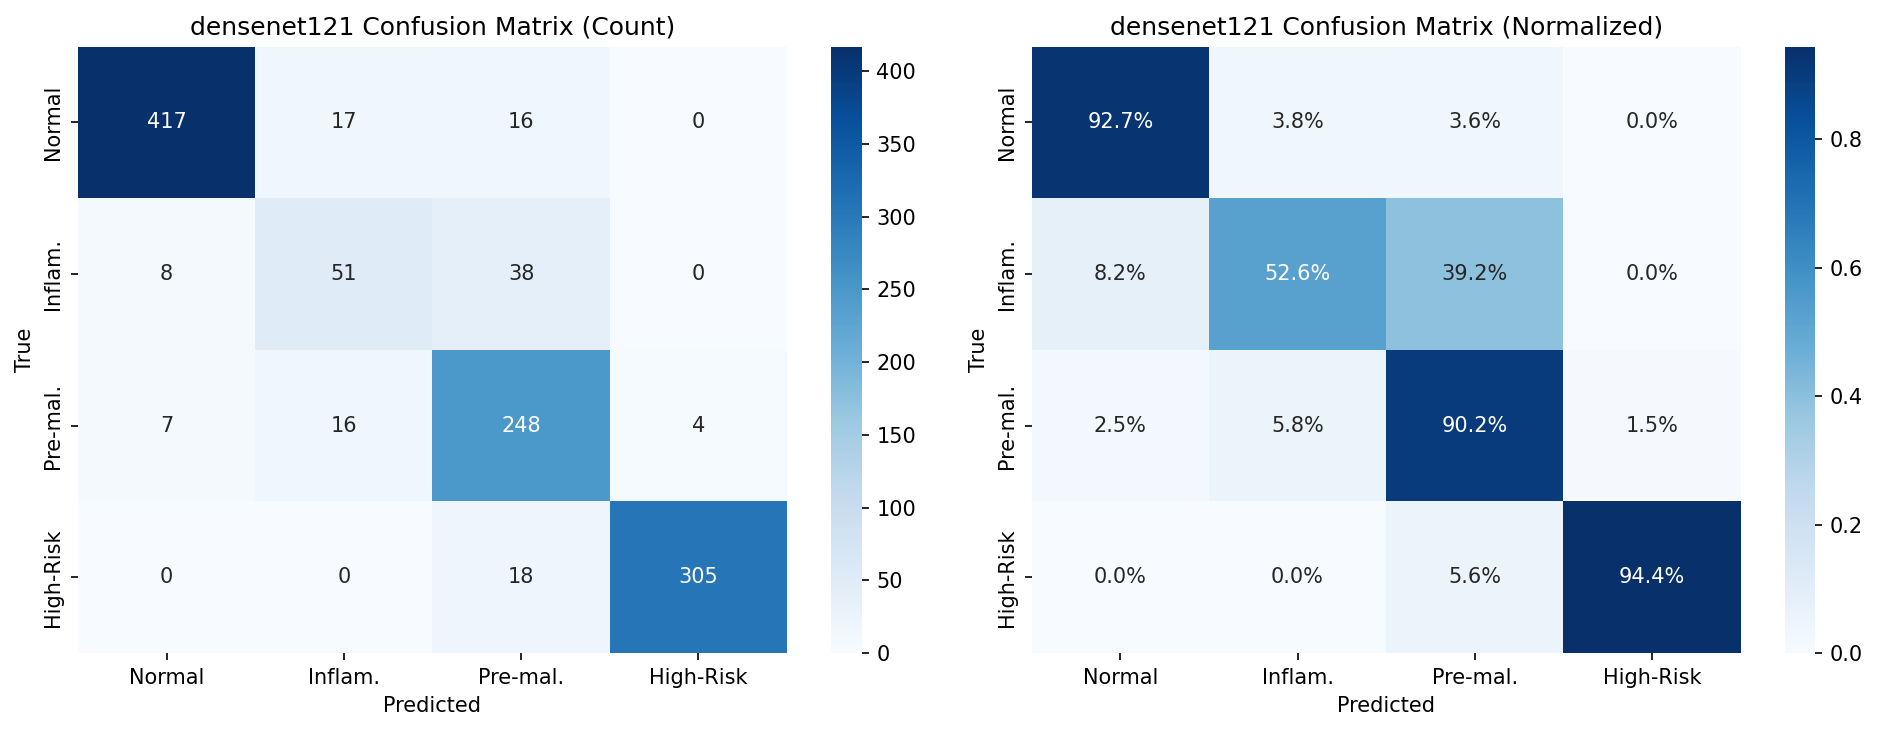
\includegraphics[width=\linewidth]{confusion_matrix_densenet121.png}
    \caption{DenseNet-121}
  \end{subfigure}
  \hfill
  \begin{subfigure}[b]{0.32\textwidth}
    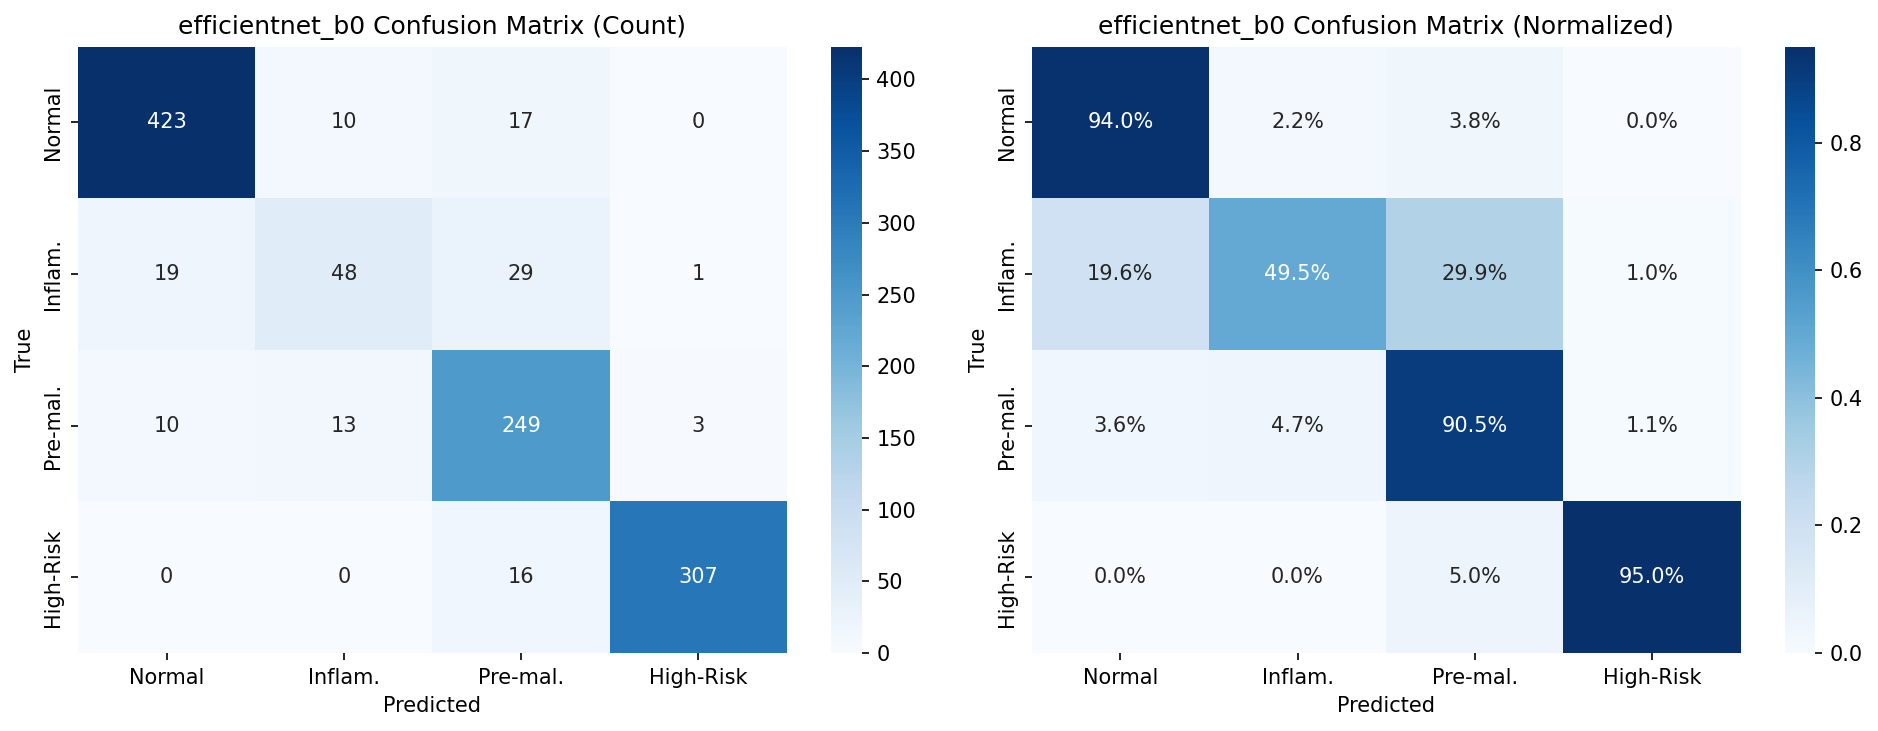
\includegraphics[width=\linewidth]{confusion_matrix_efficientnet_b0.png}
    \caption{EfficientNet-B0}
  \end{subfigure}
  \hfill
  \begin{subfigure}[b]{0.32\textwidth}
    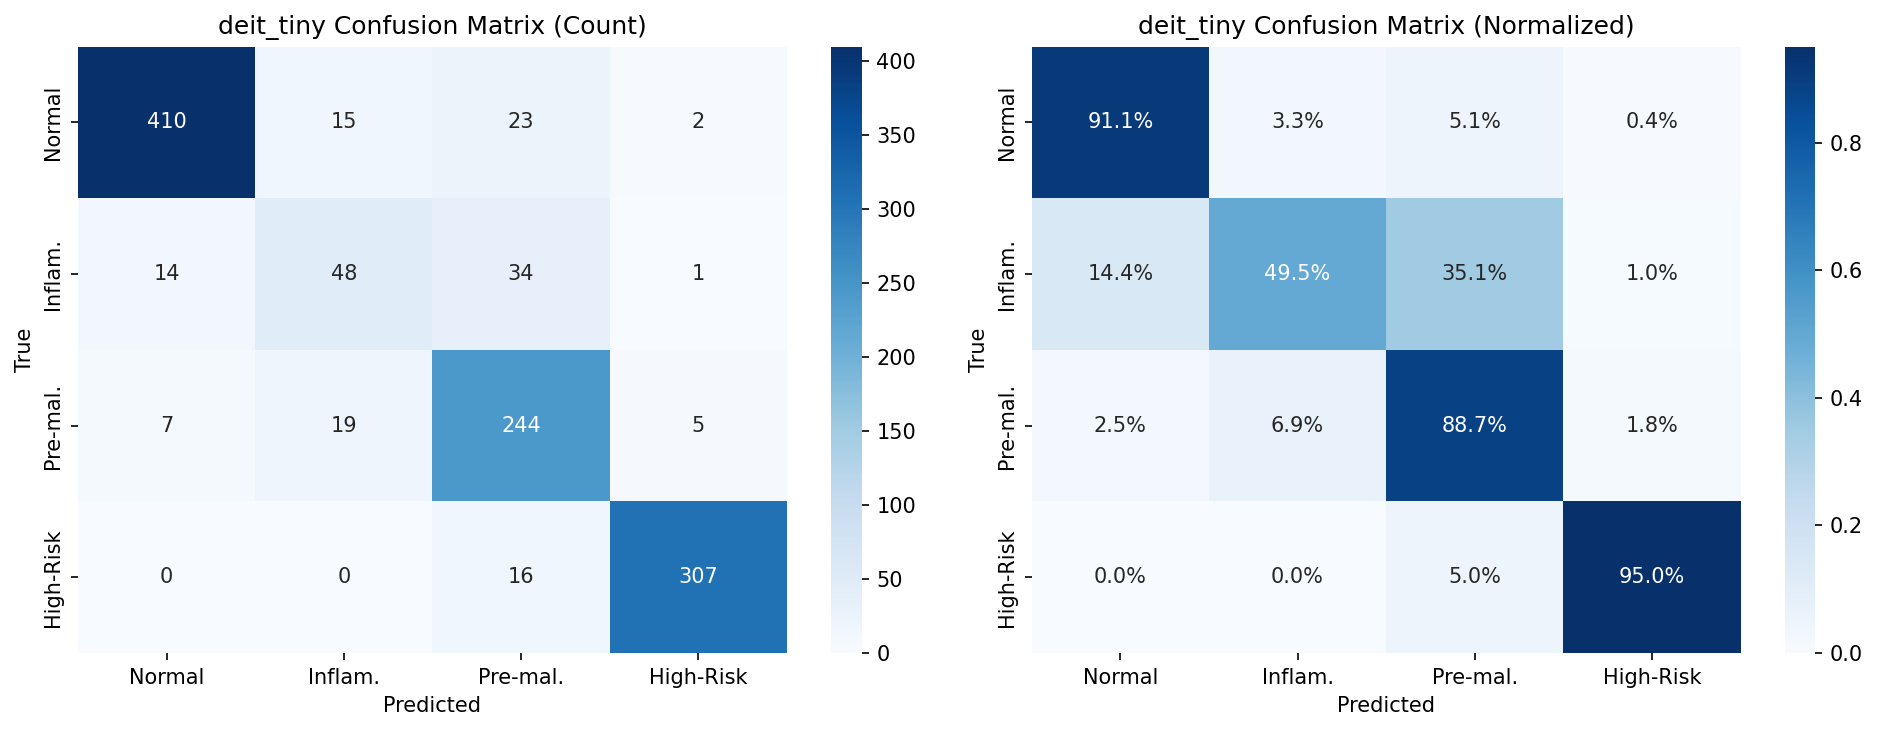
\includegraphics[width=\linewidth]{confusion_matrix_deit_tiny.png}
    \caption{DeiT-Tiny}
  \end{subfigure}
  \caption{Normalised confusion matrices on the HyperKvasir test set.
    Rows represent true labels; columns represent predicted labels.}
  \label{fig:cm}
\end{figure*}

\FloatBarrier
%% ============================================================================
\section{Discussion}
\label{sec:discussion}
%% ============================================================================

Across all three architectures, guideline-aligned four-class risk
stratification proved achievable with models containing fewer than 8\,M
parameters---hardware suitable for deployment on standard clinical
endoscopy workstations. EfficientNet-B0 led on macro F1 both in-domain
(0.8319) and zero-shot (0.7645 on Kvasir-v2), while DenseNet-121 produced
the highest mean AUC-ROC (0.9754). Perhaps most importantly from a clinical
standpoint, all three architectures achieved High-Risk recall
$\geq$\,94.4\,\% and zero missed High-Risk lesions under the MC Dropout
referral protocol---the safety outcome that motivated the AEL design.
Assigning a 5$\times$ loss penalty to High-Risk misclassification
consistently pushed models to prioritise recall on the most consequential
class without sacrificing overall accuracy.

Comparing CNN and Transformer architectures under an identical parameter
budget ($<$8\,M) isolates inductive bias rather than capacity. DenseNet-121
and EfficientNet-B0 both exploit translation invariance and hierarchical
local feature extraction, which suits mucosal texture analysis well---pit
pattern irregularity and vascular architecture are spatially compact cues.
DeiT-Tiny, by contrast, processes the image as 196 non-overlapping patch
tokens and attends globally; this may benefit lesions whose diagnosis depends
on their spatial context, such as the completeness of dyed resection margins.
In practice the performance gap between CNN and Transformer was narrow
(0.8319 vs.\ 0.8134 macro F1), suggesting that for this resolution and
dataset size, local texture remains the dominant discriminative signal.

Inspecting the GradCAM heatmaps, none of the three models appeared to latch
onto endoscope shaft reflections, text overlays, or other image artefacts.
CNN heatmaps were tighter and more focal---consistent with the local
receptive fields of convolutional filters---while DeiT-Tiny produced
broader, patch-spanning activations. For High-Risk cases, both CNN models
concentrated attention on the dye boundary in lifted-polyp images, which
aligns with how endoscopists visually assess resection completeness. Whether
the broader DeiT attention represents richer contextual reasoning or simply
lower spatial resolution in the token grid warrants further study with
higher-resolution Transformer variants.

Zero-shot performance on Kvasir-v2 dropped markedly for DenseNet-121
(0.8270\,→\,0.6415) but much less for EfficientNet-B0 (0.8319\,→\,0.7645)
and DeiT-Tiny (0.8134\,→\,0.7603). The larger DenseNet drop likely reflects
overfitting to HyperKvasir's specific colour balance and artefact
distribution; its Normal class recall fell to 55\,\% on Kvasir-v2 compared
with 94\,\% in-domain. CLAHE preprocessing normalises local contrast and
appears to assist EfficientNet-B0 and DeiT-Tiny but cannot eliminate
sensor-level domain shift. Multi-source training and feature-level domain
adaptation are natural next steps.

Patient demographic data is largely absent from publicly available GI
endoscopy benchmark datasets, including HyperKvasir. In the absence of real
annotations, CD-CTEI was computed on synthetic subgroup assignments derived
from image metadata, limiting its clinical interpretability. We report it
here as a methodological proof-of-concept rather than a definitive fairness
assessment, and explicitly caution against citing the synthetic-proxy
CD-CTEI value as evidence that the model is demographically fair in
deployment---the metric's purpose at this stage is to demonstrate that such
an audit is computable, not to certify equitable performance. Constructing
demographically annotated multi-site GI endoscopy datasets remains an open
and pressing need, particularly given evidence of differential cancer
incidence and endoscopic miss rates across age, sex, and ethnicity
subgroups~\citep{Kaminski2017}; we encourage groups with access to such data
to apply CD-CTEI as defined in Eq.~\ref{eq:cdctei} and report it as a
genuine fairness assessment.

\subsection{Inflammatory Class Performance}

Inflammatory lesions yielded the lowest per-class F1 across all three
architectures, attributable to two compounding factors. First, the
Inflammatory tier has the smallest class representation in HyperKvasir
(645 images vs.\ 1,836--3,000 for other tiers), limiting the diversity of
training examples even under WeightedRandomSampler. Second, mild inflammatory
findings---particularly early \texttt{esophagitis-a} and \texttt{hemorrhoids}
---share mucosal texture characteristics with both normal mucosa and low-grade
pre-malignant findings, creating inherent visual ambiguity at class boundaries.
This mirrors a well-documented difficulty among human endoscopists: grade-A
esophagitis under the Los Angeles classification is frequently confused with
normal mucosa even by experienced observers, so the model's difficulty on
this tier reflects a genuinely ambiguous visual boundary rather than a
correctable architectural weakness. Critically, this limitation does not
compromise clinical safety: an
Inflammatory lesion misclassified as Normal results in delayed medical
management rather than a missed resection---a qualitatively less severe
outcome than a missed High-Risk lesion. This asymmetry is precisely what the
AEL encodes, and High-Risk recall remained above 94\,\% across all
architectures regardless of Inflammatory class performance.

\subsection{Limitations}

Several limitations should be acknowledged. \emph{First}, HyperKvasir was
collected at a single institution (Baerum Hospital, Norway) using a limited
range of endoscopy systems; performance in multi-site deployments remains to
be evaluated. \emph{Second}, the four-class risk schema, while grounded in
ACG/ESGE guidelines, represents a simplification: clinical practice involves
nuanced intra-class variation (e.g., polyp histology) that cannot be
determined from optical endoscopy alone. \emph{Third}, the absence of
demographic annotations in HyperKvasir limits the clinical interpretability
of the CD-CTEI equity analysis. \emph{Fourth}, MC Dropout with $T=30$ passes
provides an approximation to Bayesian posterior inference that may
underestimate calibration uncertainty compared to ensemble methods.
\emph{Finally}, all experiments were conducted on Apple M2 MPS hardware; we
report parameter counts ($<$8\,M for all three models, Table~\ref{tab:archs})
as a proxy for deployability, but parameter count does not translate linearly
to inference latency, since memory bandwidth, operator support, and
quantisation behaviour differ substantially between MPS, embedded GPUs, and
the dedicated inference accelerators used in clinical endoscopy towers.
Frame-rate throughput on representative clinical hardware was not measured in
this study and should be characterised before any real-time deployment claim
is made.

\FloatBarrier
%% ============================================================================
\section{Conclusions}
\label{sec:conclusions}
%% ============================================================================

Three lightweight models trained with the proposed Asymmetric Endoscopy
Loss on a clinically grounded four-class risk schema demonstrate that
guideline-aligned risk stratification is achievable at under 8\,M
parameters per architecture. EfficientNet-B0 achieves macro
F1\,=\,0.8319 in-domain and 0.7645 zero-shot on Kvasir-v2; all three
architectures reach zero missed High-Risk lesions under MC Dropout
referral, with 43.9\,\% of Normal and low-confidence Inflammatory
cases auto-cleared---reducing endoscopist review burden without
compromising safety. DenseNet-121 leads on mean AUC-ROC (0.9754),
and GradCAM confirms that model attention concentrates on mucosal
features a clinician would recognise rather than imaging artefacts.

The results suggest two practical conclusions. First, the 5$\times$
High-Risk penalty in AEL is sufficient to maintain $\geq$94\,\%
High-Risk recall across architectures even when the Inflammatory class
remains difficult (F1\,=\,0.57 for EfficientNet-B0). Second, the
MC Dropout referral protocol converts a probabilistic classifier into
a structurally safe screening tool without retraining---a property
directly deployable on existing endoscopy hardware.

Three directions emerge most naturally from these results. \emph{First,
multi-site demographically annotated data:} replacing synthetic CD-CTEI
proxies with real patient demographics and validating across institutions
with different endoscopy equipment is the highest-priority open problem;
it would simultaneously resolve the equity limitation and improve
cross-dataset generalisation. \emph{Second, schema enrichment and optical
histology:} extending the four-class schema to incorporate polyp morphology
(Paris classification) and optical biopsy predictions would align the model
output more precisely with the clinical decision chain, particularly for
the Pre-malignant tier where current F1 leaves room for improvement.
\emph{Third, whole-procedure surveillance with domain-adaptive extractors:}
foundation model feature extractors, potentially combined with multiple
instance learning over full procedure frame sequences, offer a path from
single-frame classification to continuous risk surveillance across an entire
endoscopy session, with domain adaptation strategies addressing the
cross-institutional colour and sensor shift documented in the DenseNet-121
zero-shot results.

%% ============================================================================
\section*{Declarations}

\noindent\textbf{Conflict of interest}\quad The authors declare no competing
interests.

\noindent\textbf{Data availability}\quad HyperKvasir and Kvasir-v2 are
publicly available datasets. Code and trained checkpoints will be released
upon acceptance.

%% ============================================================================
\bibliographystyle{plainnat}
\bibliography{refs}

\begin{thebibliography}{99}

\bibitem[Sung et~al.(2021)]{Sung2021}
Sung H, Ferlay J, Siegel RL, et~al.
\newblock Global cancer statistics 2020: {GLOBOCAN} estimates of incidence and
  mortality worldwide for 36 cancers in 185 countries.
\newblock \emph{CA Cancer J Clin}. 2021;71(3):209--249.

\bibitem[Kaminski et~al.(2017)]{Kaminski2017}
Kaminski MF, Thomas-Gibson S, Bugajski M, et~al.
\newblock Performance measures for lower gastrointestinal endoscopy: a
  {European Society of Gastrointestinal Endoscopy (ESGE)} quality improvement
  initiative.
\newblock \emph{Endoscopy}. 2017;49(4):378--397.

\bibitem[Wang et~al.(2019)]{Wang2019}
Wang P, Berzin TM, Glissen Brown JR, et~al.
\newblock Real-time automatic detection system increases colonoscopic polyp and
  adenoma detection rates: a prospective randomised controlled study.
\newblock \emph{Gut}. 2019;68(10):1813--1819.

\bibitem[Pogorelov et~al.(2017a)]{Pogorelov2017}
Pogorelov K, Randel KR, Griwodz C, et~al.
\newblock {KVASIR}: a multi-class image dataset for computer aided
  gastrointestinal disease detection.
\newblock In: \emph{Proceedings of the ACM MMSys}; 2017. p.~164--169.

\bibitem[Shaukat et~al.(2021)]{Shaukat2021}
Shaukat A, Kahi CJ, Burke CA, et~al.
\newblock {ACG} clinical guidelines: colorectal cancer screening 2021.
\newblock \emph{Am J Gastroenterol}. 2021;116(3):458--479.

\bibitem[Ferlitsch et~al.(2017)]{Ferlitsch2017}
Ferlitsch M, Moss A, Hassan C, et~al.
\newblock Colorectal polypectomy and endoscopic mucosal resection: {European
  Society of Gastrointestinal Endoscopy (ESGE)} clinical guideline.
\newblock \emph{Endoscopy}. 2017;49(3):270--297.

\bibitem[Rawla et~al.(2019)]{Rawla2019}
Rawla P, Sunkara T, Barsouk A.
\newblock Epidemiology of colorectal cancer: incidence, mortality, survival,
  and risk factors.
\newblock \emph{Gastroenterol Rev}. 2019;14(2):89--103.

\bibitem[Tajbakhsh et~al.(2016)]{Tajbakhsh2016}
Tajbakhsh N, Gurudu SR, Liang J.
\newblock Automated polyp detection in colonoscopy videos using shape and
  context information.
\newblock \emph{IEEE Trans Med Imaging}. 2016;35(2):630--644.

\bibitem[Ebigbo et~al.(2019)]{Ebigbo2019}
Ebigbo A, Mendel R, Probst A, et~al.
\newblock Computer-aided diagnosis using deep learning for the evaluation of
  malignant potential of gastric subepithelial lesions.
\newblock \emph{Sci Rep}. 2019;9(1):4465.

\bibitem[Dosovitskiy et~al.(2021)]{Dosovitskiy2021}
Dosovitskiy A, Beyer L, Kolesnikov A, et~al.
\newblock An image is worth $16\times16$ words: transformers for image
  recognition at scale.
\newblock In: \emph{International Conference on Learning Representations};
  2021.

\bibitem[Touvron et~al.(2021)]{Touvron2021}
Touvron H, Cord M, Douze M, et~al.
\newblock Training data-efficient image transformers and distillation through
  attention.
\newblock In: \emph{Proceedings of ICML}; 2021. p.~10347--10357.

\bibitem[Liu et~al.(2021)]{Liu2021}
Liu Z, Lin Y, Cao Y, et~al.
\newblock Swin transformer: hierarchical vision transformer using shifted
  windows.
\newblock In: \emph{Proceedings of ICCV}; 2021. p.~10012--10022.

\bibitem[He et~al.(2022)]{He2022}
He K, Chen X, Xie S, et~al.
\newblock Masked autoencoders are scalable vision learners.
\newblock In: \emph{Proceedings of CVPR}; 2022. p.~16000--16009.

\bibitem[Lin et~al.(2017)]{Lin2017}
Lin TY, Goyal P, Girshick R, et~al.
\newblock Focal loss for dense object detection.
\newblock In: \emph{Proceedings of ICCV}; 2017. p.~2980--2988.

\bibitem[Borgli et~al.(2020)]{Borgli2020}
Borgli H, Thambawita V, Smedsrud PH, et~al.
\newblock {HyperKvasir}, a comprehensive multi-class image and video dataset
  for gastrointestinal endoscopy.
\newblock \emph{Sci Data}. 2020;7(1):283.

\bibitem[Pogorelov et~al.(2017b)]{Pogorelov2017b}
Pogorelov K, Randel KR, Espeland T, et~al.
\newblock Kvasir: a multi-class image dataset for computer aided
  gastrointestinal disease detection.
\newblock In: \emph{Proceedings of the 8th ACM MMSys}; 2017.

\bibitem[Reza(2004)]{Reza2004}
Reza AM.
\newblock Realization of the contrast limited adaptive histogram equalization
  ({CLAHE}) for real-time image enhancement.
\newblock \emph{J VLSI Signal Process}. 2004;38(1):35--44.

\bibitem[Huang et~al.(2017)]{Huang2017}
Huang G, Liu Z, van~der Maaten L, Weinberger KQ.
\newblock Densely connected convolutional networks.
\newblock In: \emph{Proceedings of CVPR}; 2017. p.~4700--4708.

\bibitem[Tan \& Le(2019)]{Tan2019}
Tan M, Le QV.
\newblock {EfficientNet}: rethinking model scaling for convolutional neural
  networks.
\newblock In: \emph{Proceedings of ICML}; 2019. p.~6105--6114.

\bibitem[Loshchilov \& Hutter(2019)]{Loshchilov2019}
Loshchilov I, Hutter F.
\newblock Decoupled weight decay regularization.
\newblock In: \emph{International Conference on Learning Representations};
  2019.

\bibitem[Selvaraju et~al.(2017)]{Selvaraju2017}
Selvaraju RR, Cogswell M, Das A, et~al.
\newblock {Grad-CAM}: visual explanations from deep networks via
  gradient-based localization.
\newblock In: \emph{Proceedings of ICCV}; 2017. p.~618--626.

\bibitem[Gal \& Ghahramani(2016)]{Gal2016}
Gal Y, Ghahramani Z.
\newblock Dropout as a {Bayesian} approximation: representing model uncertainty
  in deep learning.
\newblock In: \emph{Proceedings of ICML}; 2016. p.~1050--1059.

\bibitem[Jahanifar et~al.(2025)]{Jahanifar2025}
Jahanifar M, Raza M, Xu K, et~al.
\newblock Domain generalization in computational pathology: survey and
  guidelines.
\newblock \emph{ACM Comput Surv}. 2025;57(11).

\end{thebibliography}

\end{document}
